\documentclass{article}
\usepackage[english]{babel}
\usepackage[utf8]{inputenc}
\usepackage{fancyhdr}
\usepackage[margin=1in]{geometry}
\usepackage{mathtools}
\usepackage{amssymb}
\usepackage{bm}
\usepackage{amsthm}
\usepackage{blindtext}
\usepackage{natbib}
\usepackage{xcolor}
\usepackage{graphicx}
\usepackage{mathrsfs}

\usepackage{tikz}
\setcounter{subsection}{-1}
\newcommand{\N}{\mathbb{N}}
\newcommand{\R}{\mathbb{R}}
\newcommand{\Q}{\mathbb{Q}}
\newcommand{\x}{\mathbf{x}}
\newcommand{\y}{\mathbf{y}}
\newcommand{\Z}{\mathbb{Z}}
\newcommand{\norm}[1]{\left\lVert#1\right\rVert}
\newcommand{\LL}{\mathcal{L}}
\newcommand{\Prr}[1]{\text{Pr}\left(#1\right)}


\theoremstyle{definition}
\newtheorem{proposition}{Proposition}[section]
\newtheorem{theorem}{Theorem}[section]
\newtheorem{lemma}{Lemma}[section]
\newtheorem{definition}{Definition}[section]
\newtheorem{corollary}{Corollary}[section]
\newtheorem{ex}{Exercise}[section]
\newtheorem{note}{Notation}
\newtheorem{example}{Example}[section]
\newtheorem{remark}{Remark}[section]
\usepackage{cleveref}
\title{Real Analysis}
\author{Noah Jussila}
\date{\today}

\begin{document}
	\maketitle
	\bibliographystyle{chicago}
	\tableofcontents



\section{The Real Numbers}
We begin by returning to the most basic concepts in math. What exactly is a number? We begin with the most basic possible set of numbers, and use those to define more complex sets of numbers, with our goal being to define the real numbers. Lastly, we will look at the ``size'' of these sets, and explore the concept of infinity. 
\subsection{Natural Numbers, Integers, and Rational Numbers}
First, a cursory overview of several sets of numbers is in order. It is given for the sake of exposition, and to illustrate how we define sets of numbers using previously defined sets. For the sake of time, the formal definition of the standard operations (addition, multiplication, etc.) on these sets will be forgone. Rest assured that the operations we are all familiar with are well defined on these sets, and this can be shown rigorously. An excellent reference for this within the context of real analysis can be found in \cite{tao2006analysis}, who takes nothing as given. 

 The most basic numbers are those we use to count. We will call these natural numbers. \begin{definition}
Define the set $ \N\coloneqq\{0,1,2,\ldots\} $ to be the \textit{{\color{red} natural numbers}}. 
\end{definition}
\noindent The operations of addition and multiplication are well defined on $ \N $, in that when adding or multiplying natural numbers, the result is a natural number. A more succinct way of putting this is saying that $ \N $ is \textit{closed} under addition and multiplication. While the natural numbers are great for things such as counting (a fact we will return to), it fails to be useful for much more. In particular, two basic operations we are familiar with are not well defined on $ \N $.
\begin{example}\label{ex1}
	Suppose we want to find the difference in $ 2 $ and $ 5 $, both elements in $ \N $. The difference in question would be $ 2-5 $, but this is not an element of $ \N $! 
\end{example}

In order to address this shortcoming, we need to broaden our view. In effect, we need to ``add more'' numbers to $ \N $. We want to enlarge the set of natural numbers by the amount necessary for subtraction to be well defined. This can be done by taking the set of all differences of natural numbers. For all intents and purposes, this is how we define the integers. 
\begin{definition}
	Define the set $ \Z\coloneqq\{a-b\mid(a,b)\in\N^2\} $ to be the \textit{\color{red}integers}. Two integers are equal, $ a-b=c-d $, if and only if $ a+d=b+c $.\footnote{The added specification of when integers are equal can be avoided by defining $ \Z $ to be a set of equivalence classes. The equivelence relation $ \sim $ would be defined on $ \N $ as $ (a,b)\sim(c,d) $ when $ a+c=b+d $.}  
\end{definition}
\noindent We will take the ordering of $ \Z $, the negation of elements of $ \Z $, and all arithmetic properties of $ \Z $ to be given. There are two things worth noting. The first is that $ \N\subset\Z $. The identity element $ 0\in\N $ gives $ a-0=a $ for each $ a\in\N $, so any natural number can be written as the difference of two natural numbers. Secondly, we defined $ \Z $ only by using $ \N $. This is crucial, as we will define the rationals only by using $ \Z $, and in turn define the real numbers only by using the rationals.

While subtraction is well defined for $ \Z $, the same does not hold for division. 
\begin{example}
 Take the integers $ -3 $ and 6, and suppose we are interested in the ratio of the prior to the latter. Obviously, $$ \frac{-3}{6}=-\frac{1}{2} ,$$ but this is not an element of $ \Z $. 
\end{example}
We can now ``extend'' the integers to accommodate for division, in a similar fashion to when we defined the integers using the natural numbers. 
\begin{definition}
	Define the set $ \Q\coloneqq\{a/b\mid(a,b)\in\Z^2,\ b\neq0\} $ to be the \textit{\color{red}rational numbers}. Two rational numbers are equal, $ a/b=c/d $, if and only if $ ad=bc $.\footnote{Again we could use equivalence classes to define $ \Q $. The equivelence relation $ \sim $ would be defined on $ \N $ as $ (a,b)\sim(c,d) $ when $ ad=bc $.}  
\end{definition}
\subsection{``Holes'' in $ \Q $}
We now begin where the canonical \cite{rudin1964principles} opens. Our goal has been, and continues to be, to define the most comprehensive set of numbers possible. It may help to visualize what we have done so far with a number line. We can illustrate any ``gaps'' or ``holes'' by using red. This can be seen in Figure 1. 
	\begin{figure}[h]
	\centering
	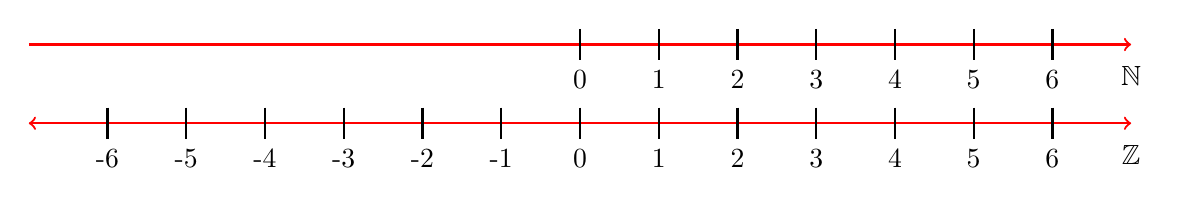
\begin{tikzpicture}
	\draw[thick, red, ->] (0,0) -- (14,0);
	\draw[thick] (7,.2) -- (7,-.2) node[anchor=north] {0};
	\draw[thick] (8,.2) -- (8,-.2) node[anchor=north] {1};
	\draw[thick] (9,.2) -- (9,-.2) node[anchor=north] {2};
	\draw[thick] (10,.2) -- (10,-.2) node[anchor=north] {3};
	\draw[thick] (11,.2) -- (11,-.2) node[anchor=north] {4};
	\draw[thick] (12,.2) -- (12,-.2) node[anchor=north] {5};
	\draw[thick] (13,.2) -- (13,-.2) node[anchor=north] {6};
	\draw (14,-.4) node {$ \N $};
		\draw[thick, red, <->] (0,-1) -- (14,-1);
		\draw[thick] (1,-.8) -- (1,-1.2) node[anchor=north] {-6};
		\draw[thick] (2,-.8) -- (2,-1.2) node[anchor=north] {-5};
		\draw[thick] (3,-.8) -- (3,-1.2) node[anchor=north] {-4};
		\draw[thick] (4,-.8) -- (4,-1.2) node[anchor=north] {-3};
		\draw[thick] (5,-.8) -- (5,-1.2) node[anchor=north] {-2};
		\draw[thick] (6,-.8) -- (6,-1.2) node[anchor=north] {-1};
	\draw[thick] (7,-.8) -- (7,-1.2) node[anchor=north] {0};
	\draw[thick] (8,-.8) -- (8,-1.2) node[anchor=north] {1};
	\draw[thick] (9,-.8) -- (9,-1.2) node[anchor=north] {2};
	\draw[thick] (10,-.8) -- (10,-1.2) node[anchor=north] {3};
	\draw[thick] (11,-.8) -- (11,-1.2) node[anchor=north] {4};
	\draw[thick] (12,-.8) -- (12,-1.2) node[anchor=north] {5};
	\draw[thick] (13,-.8) -- (13,-1.2) node[anchor=north] {6};
	\draw (14,-1.4) node {$ \Z $};
	\end{tikzpicture}
	\caption{The natural numbers and integers ordered number lines.}
\end{figure}
Clearly the natural numbers and integers are not ``comprehensive'' in that they have many gaps. This is what led us to define the rational numbers $ \Q $. It isn't immediate just how well the rationals do at covering the holes in the integers. We can get a sense of this by introducing a property of the rationals. 
\begin{proposition}{(Interspersing of integers by rationals)}\label{prop1}
	For any $ x,y\in\Q $ where $ x<y $, there exists a third rational number $ z\in\Q $ such that $ x<z<y $.
\end{proposition}
\begin{proof}
	Let there be two rationals $ x,y\in\Q $ such that $ x<y $. We can define the third rational number of interest as $ z=(x+y)/2 $. We can show that $ x<z<y $ by using arithmetic.
	\begin{align*}
		x&<y\\\frac{x}{2}&<\frac{y}{2}\\\frac{x}{2}+\frac{y}{2}&<\frac{y}{2}+\frac{y}{2}\\z&<y
	\end{align*} 
	And we can arrive at $ x<z $ by adding $ x/2 $ to each side of the given inequality.
	\begin{align*}
	x&<y\\\frac{x}{2}&<\frac{y}{2}\\\frac{x}{2}+\frac{x}{2}&<\frac{y}{2}+\frac{x}{2}\\x&<z
	\end{align*} 
\end{proof}
\begin{example}\label{ex3}
Take the rational numbers $ 0 $ and $ 1 $. Using the construction given in the previous proof we have $$ \frac{0+1}{2}=\frac{1}{2}$$ is between 0 and 1. We can now repeat this process using the pairs $ (0,1/2) $ and $ (1/2,1) $. \begin{align*}
	\frac{0+1/2}{2}=\frac{1}{4}\\\frac{1/2+1}{2}=\frac{3}{4}
\end{align*}
We could repeat this process an infinite number of times, in effect ``filling in'' gaps in $ \Z $ by successively taking the average of two rational numbers. Figure 2 shows this process on the unit interval in the rationals. 
\begin{figure}[h]
	\centering
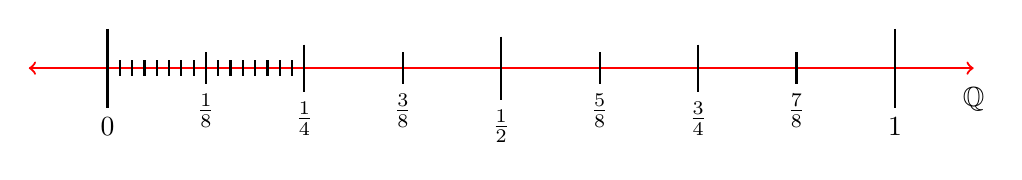
\begin{tikzpicture}
\draw[thick, red, <->] (-1,0) -- (11,0);
\draw[thick] (0,.5) -- (0,-.5) node[anchor=north] {0};
\draw[thick] (5,.4) -- (5,-.4) node[anchor=north] {$ \frac{1}{2} $};
\draw[thick] (2.5,.3) -- (2.5,-.3) node[anchor=north] {$ \frac{1}{4} $};
\draw[thick] (7.5,.3) -- (7.5,-.3) node[anchor=north] {$ \frac{3}{4} $};
\draw[thick] (8.75,.2) -- (8.75,-.2) node[anchor=north] {$ \frac{7}{8} $};
\draw[thick] (1.25,.2) -- (1.25,-.2) node[anchor=north] {$ \frac{1}{8} $};
\draw[thick] (6.25,.2) -- (6.25,-.2) node[anchor=north] {$ \frac{5}{8} $};
\draw[thick] (3.75,.2) -- (3.75,-.2) node[anchor=north] {$ \frac{3}{8} $};
\draw[thick] (10,.5) -- (10,-.5) node[anchor=north] {1};
\draw[thick] (0.15625,.1) -- (0.15625,-.1);
\draw[thick] (0.3125,.1) -- (0.3125,-.1);
\draw[thick] (0.625,.1) -- (0.625,-.1);
\draw[thick] (0.46875,.1) -- (0.46875,-.1);
\draw[thick] (0.78125,.1) -- (0.78125,-.1);
\draw[thick] (0.9375,.1) -- (0.9375,-.1);
\draw[thick] (1.09375,.1) -- (1.09375,-.1);
\draw[thick] (1.40625,.1) -- (1.40625,-.1);
\draw[thick] (1.5625,.1) -- (1.5625,-.1);
\draw[thick] (1.71875,.1) -- (1.71875,-.1);
\draw[thick] (1.875,.1) -- (1.875,-.1);
\draw[thick] (2.03125,.1) -- (2.03125,-.1);
\draw[thick] (2.1875,.1) -- (2.1875,-.1);
\draw[thick] (2.34375,.1) -- (2.34375,-.1);
\draw (11,-.4) node {$ \Q $};

\end{tikzpicture}
\caption{}
\end{figure}\\
The key question is whether or not this fills \textit{all} the gaps in the integers.
\end{example}
While \cref{ex3}, and more formally \cref{prop1}, may lead us to believe that the rational numbers have no gaps, this is unfortunately not the case. There are two classic examples that arise from two of the most basic geometric constructions. 
\begin{example}\label{ex4}
	Suppose we have a circle with diameter $ d $ and circumference $ c $. In this case, the ratio give by $ c/d $ is not an element of the rational numbers. This familiar ratio is written as $ \pi $. For the moment, we can take this as fact. We have not yet developed the tools required to proof that $ \pi\notin\Q $, but we will return to this.  
\end{example}
\begin{example}\label{ex5}
	Suppose there is an isosceles right triangle with legs of length 1, as shown in Figure 3. We want to find the length of the hypotenuse $ x $. 
	\begin{figure}[h]
		\centering
		\begin{tikzpicture}
		\draw[thick] (0,0) -- (8,0);
		\draw[thick] (0,0) -- (0,8);
		\draw[thick] (8,0)--(0,8);
		\draw[thick] (0,0) rectangle (.5,.5);
		\draw[thick] (4,.2)--(4,-.2)node[anchor=north]{1};
		\draw[thick] (.2,4)--(-.2,4)node[anchor=east] {1};
		\draw (4.3,4.3) node {$ x $};
		\end{tikzpicture}
		\caption{}
	\end{figure}\\
This is a simple application of the Pythagorean Theorem. \begin{align*}
	1^2+1^2&=x^2\\2&=x^2
\end{align*}
But this equation has no rational solution, something we can formally prove. 
\end{example}
\begin{proposition}
	There exists no rational number $ x $ which satisfies $ x^2=2 $. 
\end{proposition}
\begin{proof}
	For the sake of contradiction, suppose that there exists a rational $ x $ which satisfies $ x^2=2 $. If this were the case, we could write $ x=m/n $ for some $ m,n\in\Z $, where $ m $ and $ n $ are not both even.\footnote{Otherwise we could write $ x $ in simpler terms as $ m $ and $ n $ would have a common factor of 2.}
\end{proof}
Any $ x $ which does satisfy $ x^2=2 $ would be \textit{irrational}, in that it is not an element of $ \Q $. 
\begin{definition}
	A number is {\color{red}\textit{irrational}} if it is not an element of $ \Q $. 
\end{definition}
\noindent There are \textit{many} irrational numbers, each of which is a gap in the rationals (see Figure 4). 
	\begin{figure}[h]
	\centering
	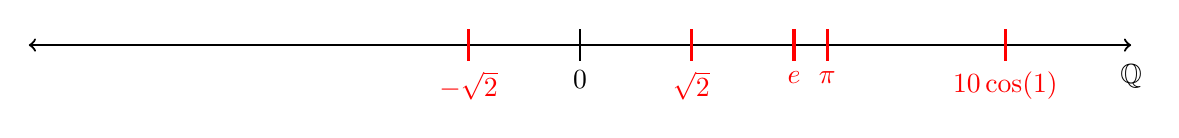
\begin{tikzpicture}
	\draw[thick] (7,.2) -- (7,-.2) node[anchor=north] {0};
	\draw[thick, black, <->] (0,0) -- (14,0);
	\draw (14,-.4) node {$ \Q $};
	\draw[very thick, red ] (10.1415,.2) -- (10.1415,-.2) node[anchor=north] {\color{red}$ \pi $};
	\draw[very thick, red ] (8.4142,.2) -- (8.4142,-.2) node[anchor=north] {\color{red}$ \sqrt{2} $};
	\draw[very thick, red ] (5.5858,.2) -- (5.5858,-.2) node[anchor=north] {\color{red}$ -\sqrt{2} $};
	\draw[very thick, red ] (9.7182,.2) -- (9.7182,-.2) node[anchor=north] {\color{red}$ e $};
		\draw[very thick, red ] (12.403,.2) -- (12.403,-.2) node[anchor=north] {\color{red}$ 10\cos(1) $};
	\end{tikzpicture}
			\caption{}
\end{figure}\\
Our goal now becomes defining a set of numbers that includes not only the rationals, but also all of the irrationals. We began with the natural numbers, and then defined a set $ \Z $ which included the additive inverses of the natural numbers. Then we filled more of the gaps in the integers by taking the ratios of integers. We are now faced with the task of defining a set which eliminates the gaps caused by irrational numbers, and doing so eniterly with the set $ \Q $. 
\subsection{$ \sup $ and $ \inf $}
Before informally constructing the real numbers, it is worth thinking about why $ \Q $ has these ``holes'', and how it relates to a specific property of sets. It goes without saying that, all the sets of numbers we've discussed up until now have some ordering to them. We can make this formal by defining an ordered set.
\begin{definition}
	An \textit{\color{red}ordered set} is some set $ S $ with a binary relation, denoted by $ < $,\footnote{In this case, ``<'' can mean \textit{any} order. It just so happens that we use the same symbol as the familiar ``less than'' order, because it is the canonical example of such a relation.} which satisfies the following properties:
	\begin{enumerate}
		\item If $ x,y\in S $, then exactly one of the statements $$x<y,\ x=y,\ y<x $$ is true.
		\item If $ x,y,z\in S $, and both $ x<y $ and $ y<z $, then $ x<z $. 
	\end{enumerate}
\end{definition}  
The statement $ ``x<y'' $ is read as ``$ x  $ is less than $ y $.''We could also write $ y>x $ instead of $ x<y $. If we were to negative $ y<x $ (``$ y $ is not less than $ x $''), we would arrive at ``y is either greater than $ x $ or equal to $ x $.'' This is denoted as $ y\ge x $. 
\begin{example}
	The set $ \Q $ is a well ordered set if we define $ < $ in the following way for $ x,y\in\Q $:
	$$ x<y\coloneqq y-x \text{ is a postiive rational number}.   $$ Note that we can only relate objects that belong to $ \Q $. This means that we have no way of comparing rational numbers and the solution to the equation $ x^2=2 $.  
\end{example}
We can use the order relation on an ordered set to define bounds on sets.
\begin{definition}
	Suppose $ S $ is an ordered set, and $ E\subset S $. If there exists a $ \beta\in S $ such that $ x\le\beta $ for all $ x\in E $, $ E $ is \textit{\color{red}bounded above}, and $ \beta $ is an \textit{\color{red} upper bound} of $ E $. 
\end{definition}
\begin{definition}
	Suppose $ S $ is an ordered set, and $ E\subset S $. If there exists a $ \beta\in S $ such that $ x\ge\beta $ for all $ x\in E $, $ E $ is \textit{\color{red}bounded below}, and $ \beta $ is a \textit{\color{red} lower bound} of $ E $. 
\end{definition}
A subtlety in both definitions that is extremely important, is that upper and lower bounds must be elements of the ordered set $ S $. The next example highlights this. 
\begin{example}
 Take $ \Z $ to be an ordered set with the natural order. Pick the subset $ E=\{-2,-1,2\}\subset \Z $. This set has many upper and lower bounds. For upper bounds we have $ 2,3,4,\ldots $. For lower bounds we have $ -2,-3,-4,\ldots
  $. It may be tempting to say that a fraction such as $ 5/2 $ is an upper bound of $ E $, but it is not. This follows from the fact that $ 5/2\notin \Z $, so we have no means of relating it to elements in $ \Z $. In this particular case, there are upper and lower bounds of the set are included in the set. This need not be the case, as the next example shows.  
\end{example}
\begin{example}
	Let's look at the ordered set $ \Q $, and subset $ E=\{x\in\Q\mid 0<x<1\}\subset \Q $.\footnote{The use of the familiar interval notation of $ (0,1) $ will be properly defined and restricted to the real numbers in the following section.} In this case, each element of $ \{x\in\Q\mid x\le 0\} $ is a lower bound of $ E $, and  each element of $ \{x\in\Q\mid x\ge 1\} $ is an upper bound of $ E $. Even though $ 0,1\notin E $, they are still least and upper bounds of $ E $ respectively. 
\end{example}
\begin{remark}
	It is often obvious what exact order we are talking about when referring to an ordered set, like in the case of $ \Q $ and $ \Z $. In these cases, we'll just assume we're using the natural order.  
\end{remark}
We now will introduce two definitions that correspond to a special type of upper and lower bound.
\begin{definition}
	Suppose $ S $ is an ordered set, $ E\subset S $, and $ E $ is bounded above. We say that $ \alpha $ is a \textit{\color{red}leas- upper-bound} of $ E $ if:
	\begin{enumerate}
		\item $ \alpha $ is an upper bound of $ E $.
		\item If $ \gamma<\alpha $, then $ \gamma $ is not an upper bound of $ E $.
	\end{enumerate}
Alternatively, we can refer to $ \alpha $ as the \textit{\color{red}supremum} of $ E $, and write $ \alpha=\sup E $
\end{definition}
\begin{definition}
	Suppose $ S $ is an ordered set, $ E\subset S $, and $ E $ is bounded below. We say that $ \alpha $ is a \textit{\color{red}greatest-lower -bound} of $ E $ if:
	\begin{enumerate}
		\item $ \alpha $ is a lower bound of $ E $.
		\item If $ \gamma>\alpha $, then $ \gamma $ is not a lower bound of $ E $.
	\end{enumerate}
	Alternatively, we can refer to $ \alpha $ as the \textit{\color{red}infimum} of $ E $, and write $ \alpha=\inf E $
\end{definition}
\begin{remark}
	Both definitions use the definite article \textit{the} before supremum and infimum. This is because they are unique. This is also implied by the use of the superlative \textit{least} and \textit{greatest}. Nevertheless, this is a result of the definition, and can be properly proven. 
\end{remark}

\begin{example}
	If we return to Example 2.7, where $ E=\{-2,-1,2\}\subset\Z $, we have $ \sup E=2 $ and $ \inf E=-2 $. 
\end{example}
\begin{example}
	In example 2.8, $ \inf E=0 $ and $ \sup E=1 $.
\end{example}
\begin{example}
	Sticking with the set $ \Q$, consider the subset $ E=\{x\in\Q\mid x^2\le 2\}\subset \Q $. This set has no supremum, because the number satisfying $ x^2=2 $ is not an element of $ \Q $ (as shown in Proposition 2.2). We will formally prove this fact shortly. 
\end{example}
It is no coincidence that a subset of $ \Q $ fails to have a supremum, because of one of the ``holes'' in $ \Q $. The following definition will help us formalize this relationship. 
\begin{definition}
	Let $ S $ be an ordered set. If for all $ E\subset S $, where $ E $ is nonempty and bounded from above, $ \sup E $ exists, then $ S $ has the \textit{\color{red}least-upper-bound} property. 
\end{definition}
The least-upper-bound property ensures that any nontrivial subset of an ordered set has a supremum in that ordered set. We could define an equivelent property known as the greatest-lower-bound property. The next two propositions serves as nice examples of the least-upper-bound property, or lack there of,  in action.
\begin{proposition}
	The set $ \Z $ has the least-upper-bound property.
\end{proposition}
The idea behind the following proof takes advantage of the fact that $ \Z $ is discrete. For some set $ E\subset \Z $, we can always just look at an upper bound of it, and keep subtracting $ 1 $ until the resulting number is in $ E $. Then we will have found our upper bound.
\begin{proof}
	We will show that an arbitrary nontrivial set $ E\subset \Z $ has a supremum. Let $ x\in E $, and $ \beta $ be an upper bound of $ E $. We know that $ \beta\ge x $ for all $ x\in E $ We can show that $ \sup E $ exists via induction on $ \beta-x $ for our arbitrary $ x\in E $. Our base case is when $ \beta-x=0 $. If this holds, then $ \beta\in E $, so $ \beta\in\Z $ and $ \sup E=\beta $. Now suppose that this statement holds when $ \beta-x=k $ for $ k\in\N $ (this is our induction hypothesis). It is either the case that $ \beta\in E $ or $ \beta\notin E $. If $ \beta\in E $, then $ \sup E=\beta $. If $ \beta \notin E $, then let $ \beta'=\beta -1 $. Then $ \beta' $ is an upper bound of $ E $, and $$\beta'-x=\beta-1-x=\beta-x-1=k+1=1=k .$$ By the induction hypothesis, $ \sup E $ exists.   
\end{proof}
\begin{proposition}
	The set $ \Q $ does not have the least-upper-bound property.
\end{proposition}
To prove this, we will first establish that $ 2 $ is an upper bound of the set defined in Example 2.11, and then show the set has no supremum via contradiction.
\begin{proof}
	If suffices to find a single subset of $ \Q $ which fails to have a supremum. Let that set be $ E=\{x\in\Q\mid x^2\le 2\} $. 
	\begin{enumerate}
		\item Suppose for contradiction that $ 2 $ is not an upper-bound of $ E $. Then there exists an $ x\in E $ such that $ x>2 $. This would imply that $ x^2>4 $, which contradicts the assumption that $ x \in E $. 
		\item Suppose for contradiction that $ E $ has a supremum, and that $ \sup E=\alpha $ for $ \alpha\in\Q $. Define a new rational number $ y\in \Q $ as 
		\begin{equation}\label{key}
		y=\alpha-\frac{\alpha^2-2}{x+2}=\frac{2(\alpha+1)}{\alpha+2}.
		\end{equation}
		Squaring this and subtracting $ 2 $ gives 
		\begin{equation}\label{key}
		y^2-2=\frac{4(\alpha+1)^2}{(\alpha+2)^2}-\frac{2(\alpha+2)^2}{(\alpha+2)^2}=\frac{2(\alpha^2-2)}{(\alpha+2)^2}.
		\end{equation} We can use $ y $ to reach a contradiction in each possible case, those being: $ \alpha^2<2 $, $ \alpha^2=2 $, $ \alpha^2>2 $.
		\begin{enumerate}
			\item Suppose that $ \alpha^2<2 $. This means that $ \alpha^2-2<0 $, so Equation (1) implies that $ y>\alpha $. At the same time, Equation (2) implies that $ y^2-2<0 $, which means $ y^2<2 $. This gives that $ y\in E $, despite the fact that $ \alpha<y $. This contradicts the fact that $ \alpha $ is an upper-bound of $ E $
			\item Suppose $ \alpha^2=2 $. We already know this cannot be the case by Proposition 2.2. 
			\item  Finally, assume that $ \alpha^2>2 $, giving $ \alpha^2-2=0 $. Equation (1)	implies $ y<\alpha $ while Equation (2) implies $ y^2-2>0 $, meaning $ y^2>2 $. This establishes $ y $ as an upper bound for $ E $, but $ y<\alpha $, which contradicts $ \sup E=\alpha $.  
	 	\end{enumerate}
	\end{enumerate}
\end{proof}
The ``holes'' in $ \Q $ are a result of $ \Q $ not having the least-upper-bound property. In order to perform calculus, we need a set that has this property, otherwise things like continuity and differentiation would not work. This property is not sufficient in and of itself though. If that were the case then we would have stopped extending out set of numbers at $ \Z $. We want a set of numbers as ``comprehensive'' as $ \Q $, but with the least-upper-bound property. It turns out, that this (and a whole lot more) is what we will get from the real numbers.  
\subsection{The Real Numbers}
We will now construct the real numbers using only $ \Q $. First, we will define the algebraic structure that the real numbers will take on.
\begin{definition}
	A \textit{\color{red}field} is a set $ F $ with two operations, addition and multiplication, which satisfy the following axioms for all $ x,y,z\in F $:
	\begin{enumerate}
		\item Axioms for addition:
		\begin{enumerate}
			\item $ x+y\in F $ (closed under addition)
			\item $ x+y=y+x $ (commutative)
			\item $ (x+y)+z=x+(y+z) $ (associative)
			\item There exists an element $ 0\in F $ such that $ 0+x=x $ (identity element)
			\item There exists an element $ -x\in F $ such that $ x+(-x)=0 $ (inverse element)
		\end{enumerate}
		\item Axioms for multiplication:
		\begin{enumerate}
			\item $ xy\in F $ (closed under multiplication)
			\item $ xy=yx $ (commutative)
			\item $ (xy)z=x(yz) $ (associative)
			\item There exists an element $ 1\in F $ such that $ 1x=x $ (identity element)
			\item If $ x\neq 0 $, there exists an element $ 1/x\in F $ such that $ x(1/x)=1 $ (inverse element)
		\end{enumerate}
		\item The distributive property:
		$$ x(y+z)=xy+xz$$
	\end{enumerate}
\end{definition}
The study of fields is its own entire subject in math, and lives within the discipline if abstract algebra. For more details about fields, see \cite{dummit2004abstract}. These axioms can be used to reach several familiar conclusions about arithmetic in fields, and can be found as formal propositions in \cite{rudin}. A more specific type of field is that which is also an ordered set.
\begin{definition}
	An \textit{\color{red} ordered field} is a field $ F $ such that
	 \begin{enumerate}
		\item $ x+y<x+z $ if $ x,y,z\in F $ and $ y<z $,
		\item $ xy>0 $ if $ x,y\in F $, $ x>0 $, and $ y>0 $. 
	\end{enumerate}
\end{definition}
\begin{example}
	The set $ \Q $ is an ordered field. 
\end{example}

Our goal is now to construct an ordered field which not only contains $ \Q $, but also has the least-upper-bound property. In order to do this we'll use the fact that $ \Q $ has ``holes'' in it. We'll form a pair of set $ (A,B) $ that partition $ \Q $ such that each of these partitions corresponds to a real number. 

\begin{definition}
	A \textit{\color{red}Dedekind cut} $ x=(A,B) $ is a pair of subsets $ A,B\subset \Q $ satisfying the following:
	\begin{enumerate}
		\item $ A\cup B=\Q $, $ A\cap B=\emptyset $, $ A\neq\emptyset $, and $ B\neq\emptyset $.
		\item If $ a\in A $ and $ b\in B $, then $ a<b $.
		\item $ A $ contains no largest element.
	\end{enumerate}
\end{definition} 
\begin{example}
	Let $ A=\{y\in \Q \mid y<0\} $ and $ B=\{y\in\Q\mid y\ge 0\} $. Our cut is $ x=(A,B) $, and can be seen in Figure 5.
		\begin{figure}[h]
		\centering
		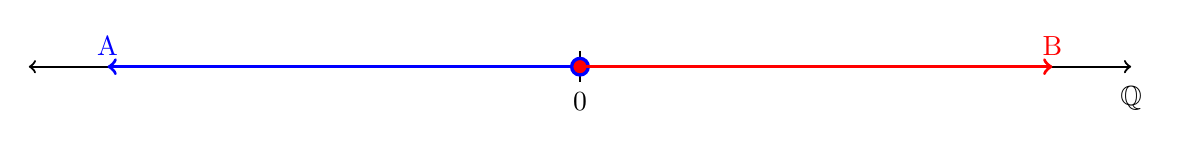
\begin{tikzpicture}
		\draw[thick] (7,.2) -- (7,-.2) node[anchor=north] {0};
		\draw[thick, black, <->] (0,0) -- (14,0);
		\draw (14,-.4) node {$ \Q $};
		\draw[ very thick, blue, ->] (7,0) -- (1,0) node[anchor=south] {A};
		\filldraw[color=blue, fill=red, very thick] (7,0) circle (3pt);
		\draw[ very thick, red, ->] (7,0) -- (13,0) node[anchor=south] {B};
		
		\end{tikzpicture}
		\caption{Dedekind cut corresponding to $ 0\in\Q $.}
	\end{figure}
This cut uniquely represents $ 0\in\Q $, as no other cut can be defined in this way ``at'' $ 0 $. 
\end{example}
\begin{example}
	Perhaps a better example is the cut defined by $ A=\{q\in\Q\mid q\le 0\text{ or }q^2<2 \} $ and $ A=\{q\in\Q\mid q> 0\text{ or }q^2>2 \} $. This cut corresponds to the solution of the equation $ x^2=2 $.  
\end{example}
\begin{definition}
	A \textit{\color{red}real number} is a Dedekind cut in $ \Q $. The set of real numbers is denoted by $ \R $. 
\end{definition}
\begin{definition}
	A real number $ x=(A,B) $ is a \textit{\color{red}rational number} if $ B $ contains a smallest element (namely $ x $).
\end{definition}
\begin{definition}
	A real number $ x=(A,B) $ is a \textit{\color{red}irrational number} if $ B $ contains no smallest element.
\end{definition}
\begin{example}
	The cut defined by $ A=\{y\in \Q \mid y<0\} $ and $ B=\{y\in\Q\mid y\ge 0\} $ is rational, as $ B $ has a smallest element in the form of $ 0 $.  
\end{example}
\begin{example}
	The cut defined by $A=\{q\in\Q\mid q\le 0\text{ or }q^2<2 \} $ and $ A=\{q\in\Q\mid q> 0\text{ or }q^2>2 \} $ has no smallest element. Therefore it is an irrational number. We will denote this particular number as $ \sqrt{2} $. 
\end{example}
Now that we have properly defined $ \R $, we can \textit{finally} refer to the quantity $ \sqrt{2} $! It is no longer a mysterious solution to an equation, and is well defined in $ \R $. This is a relatively small payoff, but the real rewards are the two following theorems. These are the main results of this section, and are of the utmost importance. The first will allow us to perform operations on $ \R $, and the second will play a key role in proving familiar theorems from calculus. The proof of the first result is rather long, and not very informative, so it is omitted. It is important to understand \textit{how} it would be proved though. Before the big reveal, we will define an order on $ \R $
\begin{definition}
	Given real numbers $ x=(A,B) $ and $ y=(C,D) $, we define the following order:$$x\le y\coloneqq A\subset C .$$ The inequality is strict if $ A\subset C $. 
\end{definition}
\begin{example}
	Let $ x=2=(A,B)=(\{y\in \Q \mid y<2\},\{y\in\Q\mid y\ge 2\})$, and $ y=3=(C,D)=(\{z\in \Q \mid z<3\},\{z\in\Q\mid z\ge 3\})$. It should come as no surprise that $ 2<3 $, but this is because $ A\subset C $.  
\end{example}
\begin{theorem}
	The set $ \R $ is an ordered field containing $ \Q $.
\end{theorem}
\begin{proof}
	See the appendix of chapter 1 in \cite{rudin}. The idea is that addition and multiplication of cuts must be define, and the all the axioms of fields and ordered fields must be verified using the cut definition of a real number. 
\end{proof}
\begin{theorem}[Completeness of the real numbers]
	The set $ \R $ has the least-upper-bound property.
	\begin{proof}
	We will show an arbitrary nonempty subset of $ \R $ has a supremum. Let $ E\subset \R $, where $ A\neq\emptyset $, have the upper bound $ \beta\in\R $. We may write $ \beta $ as a Dedekind cut, $ \beta=(A,B) $. Additionally, we may express each $ \alpha\in E $ as a cut $ \alpha=(L_\alpha,U_\beta) $. Now we will construct a real number by taking the union of all $ L_\alpha $.
	$$ \gamma=\left(\bigcup_{\alpha\in E}L_\alpha,\Q\backslash \bigcup_{\alpha\in E}L_\alpha\right)=(L,\Q\backslash
	 L)=(L,U)$$  
	I claim that $ \sup E=\gamma $.
	
	First we must verify that $ \gamma\in\R $ by showing that $ (L,U) $ is a valid Dedekind cut, and satisfies the requirements of Definition 2.13: 
	\begin{enumerate}
		\item The set $ E $ is nonempty, so there exists at least one $ \alpha=(L_\alpha,U_\alpha)\in E $. Because $ L_\alpha\neq\emptyset $ and $ U_\alpha\neq\emptyset $ by definition 2.13, we have $ L\neq\emptyset $ and $ U\neq\emptyset $. By the definition of $ U $ as $ \Q\backslash L $, we have that $  L\cup U=\Q$ and $ L\cap U=\emptyset $. 
 		\item {\color{red}FINISH THIS} 
		\item  {\color{red}FINISH THIS} 
	\end{enumerate}
	\end{proof}
Therefore $ \gamma\in\R $. By construction, $ \alpha\le\gamma $ for all $ \alpha\in E $, making $ \gamma $ an upper bound. To show that it is the least-upper-bound, we will now show any number lesser than it cannot be an upper bound. Now suppose $ \delta <\gamma $. This means $  C\subset L $, where $ \delta $ is expressed as a cut $ \delta=(C,D) $. This means there exists some $ s\in L $ such that $ s\notin C $. But $ s\in L $, so it is in $ L_\alpha $ for some $ \alpha\in E $. Hence, $ C\subset L_\alpha $, giving $ \delta <\alpha $. This shows that $ \delta $ is not an upper bound, meaning $ \sup E =\gamma$.
\end{theorem}
\begin{example}
	Consider the set of real numbers $ E=\{-1,-1/2,-1/3,-1/4,\ldots\} $. What is the supremum of this set? Intuitively, it should be $ 0 $, but we can verify this by constructing it like we did in the previous proof. Each number in $ E $ corresponds to a cut $ (L_n,U_n) $, for $ L_n=\{x\in\Q\mid x<-1/n\} $ and $ U_n=\{x\in\Q\mid x\ge -1/n\} $, where $ n\in\N $. Our supremum is $$\gamma=\left(\bigcup_{n\in \N}\{x\in\Q\mid x<-1/n\},\Q\backslash \bigcup_{n\in \N}\{x\in\Q\mid x<-1/n\}\right)=(\{x\in\Q\mid x<0\},\{x\in\Q\mid x\ge0\}). $$ Therefore, $ \gamma=0 $.  
\end{example}
You will often here the real numbers referred to as ``complete'' because they have the least-upper-bound property. This is because the least-upper-bound property ensures there are no `gaps'' in the real line like there are in $ \Q $. Down the road we will introduce a more formal definition of complete.

Finally, we will adopt the familiar notation of intervals in $ \R $, and add make an important addition to $ \R $. 
\begin{definition}
	We will use the following notation to refer to \textit{\color{red} intervals} of $ \R $:
	\begin{align*}
		(a,b)=\{x\in\R\mid a<x<b\}\\
		[a,b)=\{x\in\R\mid a\le x<b\}\\
		(a,b]=\{x\in\R\mid a<x\le b\}\\
		[a,b]=\{x\in\R\mid a\le x\le b\}
	\end{align*}
\end{definition}
\begin{definition}
	The \textit{\color{red}extended real number system} consists of the real field $ \R $ and two symbols: $ \infty $, and $ -\infty $. The original order of $ \R $ is preserved, and we define $$ -\infty <x<\infty$$ for all $ x\in\R $. 
\end{definition}
The extended real numbers do not form a proper field, but we can adopt some conventions for arithmetic using $ \infty $ and $ -\infty $ for $ x\in\R $:
\begin{enumerate}
	\item $ x+\infty=\infty $, $ x-\infty=-\infty $, $ x/\infty=x/-\infty=0 $. 
	\item For $ x>0 $, $ x(\infty)=\infty $, and $ x(-\infty)=-\infty $.
	\item For $ x<0 $, $ x(\infty)=-\infty $, and $ x(-\infty)=\infty $.
\end{enumerate}
\subsection{Properties of $ \R $}
The importance of Theorem 2.2 can not be understated. It is perhaps \textit{the} defining property of $ \R $, and it gives rise to numerous results in analysis. For now, we can use it to prove two additional properties of $ \R $.
\begin{theorem}[Archimedean property of $ \R $]
For $ x,y\in \R $ where $ x>0 $, there exists an $ n\in\N $ such that $ nx>y $.
\end{theorem}   
\begin{proof}
Let $ A $ be the set of all $ nx $ for $ x\in\R $ and $ n\in\N $, where $ x>0 $. For contradiction, suppose that there exists no such $ n\in\N $ such that $ nx>y $ for $ y\in\R $. This makes $ y $ an upper bound of $ A $. By the completeness of $ \R $, $ \sup A=\alpha $ exists. Since $ x>0 $, $ \alpha-x<\alpha $, and $ a-x $ is not an upper bound of $ A $. This means there exists an $ m\in\N $ such that $ a-x<mx $. But this would imply $ \alpha<mx+x=m(x+1) $, where $ (m+1)x\in A $. This contradicts the fact that $ \alpha $ is an upper bound of $ A $. 
\end{proof}
\begin{example}
	Suppose $ x=10 $ and $ y=213 $. By the Archimedean property of $ \R $, we know there exists a multiple of $ 10 $ that is greater than $ 213 $. $$ 10(22)=220>213$$  
\end{example}
\begin{theorem}[$ \Q $ is dense in $ \R $]
For $ x,y\in \R $ where $ x<y $, there exists a $ p\in\Q $ such that $ x<p<y $. 
\end{theorem}  
\begin{proof}
We have $ x<y $, giving $ y-x>0 $. By the Archimedean property (Theorem 2.3), there exists an $ n\in\N $ such that 
\begin{equation}\label{key}
n(y-x)>1.
\end{equation}
We can use Theorem 2.3 to find $ m_1,m_2\in\N $ for which:
\begin{align*}
	m_1>nx,\\m_2>-nx.
\end{align*}
We can combine these two inequalities to conclude $ -m_2<nx<m_1 $. This implies there exists an $ m\in\N $ (with $ -m_2\le m\le m_1 $) such that \begin{equation}\label{key}
m-1\le nx<m.
\end{equation}  
If we combine $ (3) $ and $ (4) $ we get $$ nx<m\le 1+nx<ny.$$ Dividing by $ n $ (which is positive) gives $ x<\frac{m}{n}<y$. 
\end{proof}
The density of $ \Q $ in $ \R $ is both surprising and useful for constructing examples. In practice, it means that every irrational number has a rational number arbitrarily close to it. We can approximate any number in $ \R $ arbitrarily well with a rational number.
\begin{example}
We will now mimic the proof of Theorem 2.4 with actual numbers. We will find a rational $ p\in\Q $ such that $ e<p<\pi $.\footnote{You shouldn't even need to perform the construction to arrive at an answer, as $ e $ and $ \pi $ are not particularly ``close'' to each other. We could for instance take $ p=3 $. } We have $ \pi-e>0 $. We know $$ 3(\pi-e)>1 .$$ Next we pick whole numbers $ m_1=9 $ and $ m_2=8 $, and get the inequality $ 8<3e<9 $. Now take $ m $ to be $ 9 $ and reach our final inequality of $$ 3e<9<1+3e <3\pi.$$ Dividing by $ n=3 $ gives our desired rational number is $ 9/3=3 $.  
\end{example}
\begin{example}
	Let $ \sqrt{2}\in\R $, and let $ \varepsilon>0 $.\footnote{This is the first time we're using the infamous $ \varepsilon $. It just stands in for any arbitrarily small positive number.} By the density of $ \Q $ in $ \R $, there exists $ p\in\Q $ such that $ \sqrt{2}-\varepsilon<p<\sqrt{2} $. This will hold \textit{for all} $ \varepsilon>0 $ so as we let $ \varepsilon $ become smaller and smaller, we will have an increasingly accurate rational approximation of $ \sqrt{2} $.
\end{example}     
\subsection{Cardinality}
So far, I've been intentional in avoiding any discussion of the size of the sets we have been working with. When constructing $ \Z $ from $ \N $, it was never stated that $ \Z $ was somehow ``bigger'' than $ \N $. All we know is that $ \Z $ has elements that $ \N $ does not. The same can be said for $ \Z $ and $ \Q $, or $ \Q $ and $ \R $. It is now time that we turn our attention to this matter, and more generally the size, or ``cardinality'' of sets. 

Determining the size of a set amounts to counting the number of elements in that set. But how do we make the notion of counting formal? We will do this with functions. Before formally defining anything, consider how you may count something. If you are tasked with counting the number of elements in the set $ X=\{a,b,c\} $, you're answer will surely by 3. How did you get that number? You said assigned the number $ 1 $ to $ a $, $ 2 $ to $ b $, and $ 3 $ to $ c $. We should note three different things about this process:
\begin{enumerate}
	\item Each number we use is from $ \N $.
	\item Each element of $ X $ is assigned a number. We wouldn't have counted properly if we skipped some element. 
	\item No number in $ \N $ is assigned to multiple elements in $ X $. We do not want to count multiple elements as a single element.
\end{enumerate}
This process of assigning elements in $ \N $ to those in $ X $ is shockingly similar to the notion of a function, as we are mapping elements from one set to those in another set. Furthermore, the properties we must obey while counting have their own analogous forms with functions: surjectivity, and injectivity. For this reason, we will use functions to formalize the size of a set.

First, we will address the abstract case of when two sets have the same number of elements, and then we will transition to the size of sets.
\begin{definition}
	The \textit{\color{red}cardinality} of a set $ X $, denoted $ |X| $, is the number of elements that belong to the set.   
\end{definition} 
\begin{definition}
	Two sets $ X $ and $ Y $ have \textit{\color{red}the same cardinal number} if there exists a bijection $ f:X\to Y $ from $ X $ to $ Y $.  
\end{definition} 
\begin{proposition}
	Define the relation $ X\sim Y $ \textit{if and only if} $ X $ and $ Y $ have the same cardinal number ($ |X|=|Y| $). The relation $ \sim $ is an equivalence relation. 
\end{proposition} 
\begin{proof}
	We have that $ X\sim X $ by letting $ f:X\to X $ be $ f(x)=x $, so $ \sim $ is reflexive. If $ X\sim Y $, there exists a bijection $ f:X\to Y $. Since $ f $ is a bijection, it has an inverse $ f^{-1}:Y\to X $. This inverse is itself a bijection, so $ Y\sim X $, making $ \sim $ symmetric. Lastly, assume $ X\sim Y $ and $ Y\sim Z $. We have bijections $ f:X\to Y $ and $ g:Y\to Z $. The composition of two bijections is a bijection, so $ h:X\to Z $ is a bijection where $ h:X\to Z $. This makes $ \sim $ transitive.  
\end{proof}
\begin{example}
	Let $ X=\{1,2,3\} $ and $ Y=\{\sqrt{2},e,\pi\} $. We can define $ f:X\to Y $ as $$ f(x)=\begin{cases}
	\sqrt{2}\text{ if }x=1\\e\text{ if }x=2\\\pi\text{ if }x=3
	\end{cases}.$$
	\begin{figure}[h!]
		\centering
		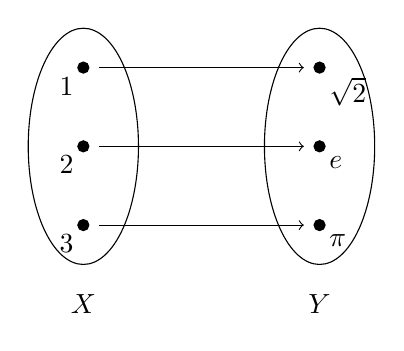
\begin{tikzpicture}
		\draw (0,0) ellipse (0.7cm and 1.5cm);
		\draw (3,0) ellipse (0.7cm and 1.5cm);
			\filldraw (0,0) circle (2pt) node[anchor=north east] {$ 2 $};
			\filldraw (0,1) circle (2pt) node[anchor=north east] {$ 1 $};
			\filldraw (0,-1) circle (2pt) node[anchor=north east] {$ 3 $};
			\filldraw (3,0) circle (2pt) node[anchor=north west] {$ e $};
			\filldraw (3,1) circle (2pt) node[anchor=north west] {$ \sqrt{2} $};
			\filldraw (3,-1) circle (2pt) node[anchor=north west] {$ \pi $};
		
			\draw (0,-2) node {$ X $};
			\draw (3,-2) node {$ Y $};
			\draw[->] (0.2,0) -- (2.8,0) ;
			\draw[->] (0.2,1) -- (2.8,1) ;
			\draw[->] (0.2,-1) -- (2.8,-1) ;
		\end{tikzpicture}
		\caption{Bijection $ f:X\to Y $.}
	\end{figure}  \\
This function is clearly a bijection, and we have that $ |X|=|Y| $.
\end{example} 
\begin{example}
	Let $ \Z^-=\{x\in\Z\mid x<0\} $ and $ \Z^+=\{x\in\Z\mid x>0\} $. There exists a very natural bijection between these sets, namely that which maps each element in $ \Z^+ $ to it's negative counterpart in $ \Z^- $. Formally, $ f:\Z^+\to\Z^- $ is define as $ f(x)=-x $. This function is clearly a bijection, and its existence shows that $ |Z^+|=|Z^-| $. There are the same number of positive integers as negative integers  
\end{example}
\begin{remark}
	Because $ f:X\to Y $ is a bijection, it doesn't matter which set is the domain and which set is the codomain. A function is invertible if and only if it is a bijection, and a functions inverse is a bijection, so we would just have $ f^{-1}:Y\to X $ if we picked the sets in the other order. In example 2.23, we could have instead assigned each negative integer to it's positive counterpart and had $ f:\Z^-\to\Z^+ $. In this case we would still have $ f(x)=-x $, as this particular function is its own inverse! 
\end{remark}

As discussed earlier, counting is intrinsically linked to the set of natural numbers $ \N $. We will now make this formal by defining three types of sets: finite sets, countably infinite sets, and uncountably infinite sets.
\begin{definition}
	A set $ X $ is \textit{\color{red}finite} if there exists a subset of the whole numbers $ N\subset \N $ for which $ X $ and $ N $ have the same cardinal number.
\end{definition} 
\begin{definition}
	A set $ X $ is \textit{\color{red}countably infinite} if $ X $ has the same cardinal number as $ \N $. Alternatively, $ X $ is countably infinite if there exists a bijection $ f:X\to\N $. This is sometimes denoted as $ |X|=\aleph_0 $.\footnote{This symbol is an ``aleph'', and is the first letter of the Hebrew alphabet.} 
\end{definition}
\begin{definition}
	A set $ X $ is \textit{\color{red}countable} if it is countably infinite or finite.
\end{definition}
\begin{remark}
	From here on out, I'm going to use countable and countably infinite interchangeably, as nearly all the sets we are interested in are infinite.  
\end{remark}
\begin{definition}
	A set $ X $ is  \textit{\color{red}uncountably infinite} (or uncountable) if it is neither finite nor countably infinite.
\end{definition}
Before jumping into examples, let's unpack some of this. Finiteness and countable infiniteness depend on whether a set has the same cardinal number as a subset of $ \N $ or $ \N $ itself. This means we can find a bijection between the set and a subset of $ \N $ or $ \N $ itself. Definition 2.22 and 2.23 are often presented in terms of this hypothetical bijection. Secondly, two of these definitions involve infinity. A set can be either countably infinite or uncountably infinite. In a sense, some infinite sets have so many elements that they cannot even be counted, and are ``bigger'' than other uncountable sets! These two concepts of infinity will show up constantly in real analysis. Hopefully examples will make this clear. Some of the following examples are so important that they will be presented as formal results. 
\begin{example}
 We will modify Example 2.22. Let Let $ X=\{\sqrt{2},e,\pi\} $ and $ N=\{1,2,3\}\subset \N$. Take our bijection to be the inverse of the function defined previously in Example 2.22. This shows that $ X $ is finite, and $ |X|=3 $. 
\end{example}
\begin{proposition}
	The set $ \N $ is countably infinite.
\end{proposition}
\begin{proof}
	Define $ f:\N\to\N $ as $ f(n)=n $. This function is clearly a bijection. 
\end{proof}
\begin{proposition}
	The set $ \Z $ is countably infinite.
\end{proposition}
Before proving this result, it's worth acknowledging that it seem paradoxical. How can it be that $ \Z $ is the same size as $ \N $, despite $ \Z $ being defined as $ \N $ plus more elements? It would make more sense for $ \Z $ to have twice the cardinality as $ \N $, but this is not the case. The result may sit better if you consider just how we would count $ \Z $. If you started at $ 1\in\Z $, followed by $ 2\in\Z $, etc. then you would miss all the negative numbers! Instead, we need to be clever in the order in which we count $ \Z $. We will instead count in the following order: $ 0,1,-1,2,-2,\ldots $. We could count like this forever and never run out of $ \N $, and never miss any elements of $ \Z $. This is why we have $ |\N|=|\Z| $. 
\begin{proof}
Recall that we can select either $ \Z $ or $ \N $ to be the domain of our bijection. We will define $ f:\N\to\Z $ as
$$f(n)=\begin{cases}
\frac{n}{2}\text{ if }n\text{ is even}\\
-\frac{n-1}{2}\text{ if }n\text{ is odd}
\end{cases}.$$
This function counts $ \Z $ in the aforementioned manner of alternating between positive and negative integers. We now will verify that $ f $ is a bijection, by showing it is injective and surjective.\footnote{It would be quicker to show $ f $ has an inverse, but that approach is not as instructive.} Let $ y\in\Z $, and pick $ x\in\N $ such that $ x=2y $ if $ y $ is even, and $ x=-2y+1 $ if $ y $ is odd. This choice of $ x\in\N $ gives $ f(x)=y $, so $ f $ is surjective. Now suppose that $ f(x_1)=f(x_2) $. If $ x_1/2=x_2/2 $, then $ x_1=x_2 $. If $ -(x_1-1)/2=-(x_2-1)/2 $, then $ x_1=x_2 $. Therefore, $ f $ is injective.
\end{proof}
An even more surprising result is that not only $ |\N|=|\Q| $, but also $ |\N|=|\Z|=|\Q| $! Even if we add every possible fraction to the integers, the size of our set remains the same.
\begin{theorem}
	The set $ \Q $ is countably infinite. 
\end{theorem}

\begin{proof}
	We can enumerate the rational numbers in the following way: $$ \frac{0}{1},\frac{1}{1},\frac{-1}{1},\frac{1}{2}, \frac{1}{3}, \frac{2}{1}, \frac{-2}{1}, \frac{-1}{3}, \frac{1}{4}, \frac{1}{5}, \frac{-1}{4}, \frac{2}{3},\ldots $$ This particular ordering can be seen in Figure 7. The red arrows in Figure 7 show the order in which we count, and it becomes evident that we will eventually count every possible fraction. Note that we only count fractions which are expressed in simplest terms, with others in gray. 
\begin{figure}[h!]
	\centering
	\includegraphics[width=0.9\linewidth]{figures/Qcountable}
	\caption{}
	\label{fig:qcountable}
\end{figure}
\end{proof}
It may not be a surprise that it is not possible to count $ \R $. This puts $ \R $ in our second category of infinite sets, uncountably infinite.
\begin{theorem}
	The set $ \R $ is uncountably infinite. 
\end{theorem}
The proof of this theorem is a classic, and is due to Cantor. 
\begin{proof}
Suppose for contradiction that $ \R $ were countably infinite. There exists a bijection $ f:\N\to\R $, and we make a table of values the function takes on (see Table 1). Table 1 is just an example of what such a bijection may look like, and the exact values are moot.
\begin{table}[h!]
	\centering
	\begin{tabular}{cc}
		$ n\in\N  $       & $ f(n)\in\R $              \\ \hline
		1        & $4.3214875\ldots$ \\
		2        & $1.4918401\ldots$           \\
		3        & $3.0194510\ldots$                   \\
		4        & $9.0194510\ldots$                  \\
		5        & $0.3917293\ldots $               \\
		6        & $ 5.9184017\ldots $\\
		7        & $ 1.9284010\ldots $                \\
		$\vdots$ & $\vdots$         
	\end{tabular}
\end{table}
Because $ f $ is a bijection, this table should go on forever, and count every element of $ \R $. To reach a contradiction, we will simply show there exists a real number that was not counted.\footnote{There in fact exist \textit{many} that would go uncounted, but it suffices to find just one.} ``Construct'' this uncounted real number in the following way: let the $ n^{th} $ digit (decimal places included) take on the value of the $ n^{th}$ digit of $ f(n) $ minus one (if it is $ 0 $, set it to $ 9 $). For Table 1, the first digit would be the first digit of $ f(1) $ minus 1, which is $ 4-1=3 $. The second digit would be the second digit of $ f(2) $ minus 1, which is $4-1=3$. We repeat this process for all $ n\in\N $, and in our case we get $$3.308690\ldots $$
By construction, the $ n^{th} $ digit of this number is different from at least one of the $ n^{th} $ digits of $ f(n) $. This holds for every $ n\in\N $, so this number is different from every value of $ f(n) $, and was therefore not counted.  
\end{proof}
\begin{corollary}
	Every infinite subset of $ \R $ is uncountable.
\end{corollary}
\begin{example}
	Every interval $ [a,b]\subset\R $ is uncountable. 
\end{example}
Now that we've seen which familiar sets are and are not countable, there are several key results involving the cardinality of sets that deserve attention. These will establish what happens to the cardinality of sets when different set operations are performed. 
\begin{proposition}
	Let $ \{E_n\} $, $ n\in\N $, be a sequence of countably infinite sets, and let $ E=\cup_{n\in N}E_n $ be a countable union. The set $ E $ is countably infinite. 
\end{proposition}
\begin{proposition}
	We will prove via induction. Our base case is $ n=2 $. The sets $ E_1 $ and $ E_2 $ are countably infinite, so there exists bijections $ f:\N\to E_1 $ and $ g:\N\to E_2 $. Without loss of generality, assume $ E_1\cap E_2=\emptyset $.\footnote{Otherwise, we could replace $ E_1 $ with $ E_1\backslash E_2 $.} Define $ h:\N\to E_1\cup E_2 $ as $$ h(k)=\begin{cases}
	f(k/2)\text{ if }k  \text{ is even}\\
		g((k+1)/2)\text{ if }k  \text{ is odd}
	\end{cases}. $$ This function counts the elements in the set by alternating between those in $ E_1 $ and $ E_2 $ (like in the proof of Proposition 2.7). The function $ h $ is a bijection, so $ E_1\cup E_2 $ is countably infinite. Now suppose this holds for $ E_1,\ldots E_{n-1} $. We can write $ E $ as a union of two countably infinite sets by taking the union over $ E_1,\ldots E_{n-1} $, which is countably infinite by the induction hypothesis. 
	\begin{align*}
		E&=\bigcup_{n\in \N} E_n\\
		 &=E_1\cup E_2\cup\cdots E_{n-1}\cup E_n\\
		 &=(E_1\cup E_2\cup\cdots E_{n-1})\cup E_n
	\end{align*} 
	Therefore $ E $ is countably infinite. 
\end{proposition}
\begin{corollary}
	If $ X $ is uncountable, and $ E\subset X $ is countably infinite, then $ X\backslash E$ is uncountably infinite.
\end{corollary}
\begin{example}
	Let $ E_n=\{m/n\mid m\in\Z\} $ for $ n\in\N $. Each $ E_n $ is countable as there is a bijection $ f_n:E_n\to\Z $ defined as $ f_n(x)=nx $, and $ \Z $ is countably infinite.\footnote{This allows us to use the transitivity of sets having the same cardinality.} Note that $$\bigcup_{n\in \N}E_n=\Q, $$ which is indeed countably infinite. 
\end{example}
\begin{example}
	The set $ \R $ is uncountable. We have that $ \Q\subset \R $ is countable. By Corollary 2.1, $ \R\backslash \Q $ (the set of irrational numbers) is uncountable. This means that in a certain sense, there are more gaps in $ \Q $ than there aren't! We are not even capable of counting all the gaps, whereas we can count $ \Q $. 
\end{example}
\begin{proposition}
	Let $ X $ be a countable set. Any subset $ Y\subset X $ is countable
\end{proposition}
\begin{proof}
	There exists a bijection $ f:\N\to X $. If we restrict the codomain of $ f $ to be $ Y $, $ f $ is still a bijection. 
\end{proof}
\begin{example}
	Every subset of $ \Q $ is countable, because $ \Q $ is countable. We already know two such examples: $ \N $ and $ \Z $. 
\end{example}
\begin{proposition}
	Let $ \{E_n\} $, $ n\in\N $, be a sequence of countably infinite sets, and let $ E=\bigtimes\limits_{n\in N}E_n $ be a countable Cartesian product. The set $ E $ is countably infinite. 
\end{proposition}
\begin{proof}
	It suffices to show the result for two sets $ E_1 $ and $ E_2 $, and then apply induction using the same argument used in the proof of Proposition 2.9. We have bijections $ f:E_1\to\N$ and $ g:E_2\to\N $. Define $ h:E_1\times E_2 $ as $$ h((a,b))=2^{f(a)}3^{g(a)},$$ where $ (a,b)\in E_1\times E_2 $. Each element in $ h(E_1\times E_2) $ is a whole number with a prime factorization comprised of only $ 2 $ and/or $ 3 $. Because each element of $ \N $ is uniquely determined by its prime factorization, $ h $ is injective. Unfortunately, $ h $ is no surjective, as there exist many elements of $ \N $ with prime factorizations that include more than $ 2 $ and/or $ 3 $. If we restrict the codomain of $ h $ to just its image, we have a bijection $ h':E_1\times E_2\to  h(E_1\times E_2) $  We do have that $ h(E_1\times E_2)\subset \N  $, so by Proposition 2.10, $ |h(E_1\times E_2)|=\aleph_0 $ . By transitivity, $ |E_1\times E_2|=\aleph_0 $. The aforementioned induction can be applied to conclude $ |E|=\aleph_0 $. 
\end{proof}
\begin{example}
	The set of all pairs of rational numbers $ \Q^2 $ is countable.
\end{example}
\subsection{Exercises}
\begin{ex}
	Show that $ \sqrt{3} $ is irrational.
\end{ex}
\begin{ex}
	Let $ (S,<) $ be an ordered set, and $ T $ be a nonempty subset of $ T $. Verify that $ T $ has at most one supremum.
\end{ex}
\begin{ex}
	Let $ E $ be a nonempty subset of an ordered set; suppose $ \alpha $ is a lower bound of $ E $ and $ \beta $ is an upper bound of $ E $. Prove that $ \alpha\le\beta $. 
\end{ex}
\begin{ex}
	Let $ E $ be a nonempty subset of $ \R $ which is bounded below. Let $ -E=\{-x\mid x\in E\} $. Show that $ \inf E=-\sup(-E) $. 
\end{ex}
\begin{ex}
	A set has the least-upper-bound property \textit{if and only if} it has the greatest-lower-bound property. 
\end{ex}


\section{Point-Set Topology in Metric Spaces}
One of the main goals of calculus is to study rates of change and limiting behavior. Both of these concepts require some notion of distance, and to that end we will study \textit{metric spaces}, sets equipped with a distance function. Any such space has induced ``topological'' properties. This is a fancy way of saying that we can use distance to categorize different types of sets. Of particular interest, will be the different types of sets in $ \R $ and $ \R^n $, as the properties these sets have will have major implications down the road.  
\subsection{Metric Spaces}
Our first definition will outline how we endow a set with some notion of distance. 
\begin{definition}
	A \textit{{\color{red}metric space}} is an ordered pair $ (M,d) $ where $ M $ is a set and $ d:M\times M\to[0,\infty] $ is a function which satisfies:
	\begin{enumerate}
		\item $ d(x,y)=0 $ $ \iff $ $ x=y$.
		\item $ d(x,y)=d(y,x) $ for all $ x,y\in M $ where $ x\neq y $.
		\item $ d(x,z)\le d(x,y)+d(y,z) $ for all $ x,y,z\in M $. (Triangle Inequality)
	\end{enumerate}
\end{definition}
The function $ d $ is often called the metric, and most of its properties are compatible with our everyday understanding of distance. Firstly, distance cannot be negative. There is no distance between a point and itself. The distance from $ x $ to $ y $ is the same from $ y $ to $ x $. The final property may not be as immediate, but it is extremely important.
 
Suppose you are traveling from point $ x $ to $ z $. If you decide to take a detour to point $ y $ before heading to $ z $, then the triangle inequality ensures that you travel a weakly greater distance. An illustration shown in Figure 8 of this gives rise to the inequalities name.
\begin{figure}[h!]
	\centering
	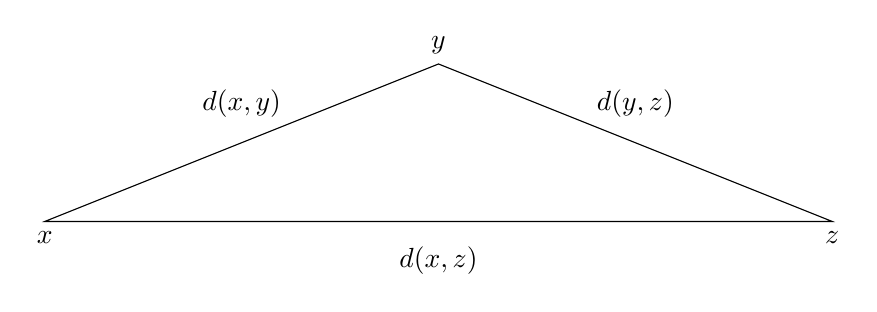
\begin{tikzpicture}
		\draw (0,0) node[anchor=north]{$x$}
		-- (10,0) node[anchor=north]{$z$}
		-- (5,2) node[anchor=south]{$y$}
		-- cycle;
		\draw (5,-0.5) node {$ d(x,z) $};
		\draw (2.5,1.5) node {$ d(x,y) $};
		\draw (7.5,1.5) node {$ d(y,z) $};
	\end{tikzpicture}
	\caption{The triangle inequality.}
\end{figure}  
Geometrically, this is equivalent to saying that the length of any side of a triangle cannot be greater than the sum of the other two lengths. Whenever presented with a weak inequality, it is often helpful to ask ``when does this hold with equality''? In this case the answer is when $ y $ is on the line segment formed by $ x $ and $ z $. In this case going to $ y $ isn't a detour at all, but just a trivial stop on the way from $ x $ to $ z $! 
\begin{example}[Euclidean Metric]
The real line $ \R $ is a metric space when equipped with the metric $ d(x,y)=|x-y| $. 
\end{example}
\begin{example}[Euclidean Metric]
Euclidean space $ \R^n $ is a metric space when equipped with the metric $$ d(\mathbf{x},\mathbf{y})=|\x-\y|=\sqrt{(x_1-y_1)^2+\cdots+(x_n-y_n)^2} .$$ The Euclidean metric is sometimes refered to as the $ \ell^2 $-metric. The Euclidean metric is intimately linked to the concept of a \textit{\color{red}norm}. Recall from linear algebra that Euclidean space is a vector space where vectors are elements of $ \R^n $, and scalers are elements of $ \R $. This space is equipped with function $ \norm{}_2:\R^n\to\R $ that measures the length of vectors. $$ \norm{\x}_2=\sqrt{x_1^2+\cdots+x_n^2}$$ We can write the $ \ell^2 -$metric as $ d(\x,\y)=\norm{\x-\y}_2 $. We'll come back to the concept of a norm throughout, and will discuss it at length when treating functional analysis.
\end{example}
\begin{example}[Taxi-Cab Metric]
If our set is $ \R^2 $ we can let $ d(\mathbf{x},\mathbf{y})=|x_1-y_1|+|x_2-y_2| $. This is often referred to as the taxi-cab metric, as it is how you would measure distance if driving a car on a grid. We can extend to $ \R^n $ and let $ d(\mathbf{x},\mathbf{y})=\sum_{i=1}^{n}|x_i-y_i| $. This metric is also called the $ \ell^1 -$metric.    
\end{example}
\begin{example}[$ p $-Adic Metric]
The previous examples are easy to verify, but this may not always be the case. Suppose are set is $ \Z $ and $ d:\Z\times\Z\to[0,\infty] $ is defined as $$ d(x,y)=\begin{cases}
0\text{ if }x=y\\p^{-\max\{m\in\N|\ p^m|(x-y) \}}\text{ otherwise}
\end{cases}$$ for some prime number $ p $. Before we verify this is a metric, it's worth getting a feel for how the metric actually works. If $ x\neq y $, then the distance between two points is $ p $ raised to some negative power. That negative power is defined to be the maximum whole number $ m $ such that $ (x-y) $ is divisble by $ p^m $. This gives us the vague idea that distance between points $ x $ and $ y $ is somehow related to how many times $ p $ shows up in the prime factorization of $ (x-y) $ (where $ m $ is the number of times). Let's take $ p=3 $, and pick several points in $ \Z $ to measure the distance between.    
\begin{center}
\begin{tabular}{cccccc}
	$ x $ & $ y $ & $ x-y $ & prime factorization of $ x-y $ & $ m $ & $ p^{-m} $ \\ \hline
	$ 100 $& 19  &  $ 81 $   &          $ 3^4 $                  &  $ 4 $  &     $ 1/81 $                  \\
$ 368 $	& 8  &  $ 360 $   &            $ 2^3\cdot5\cdot9 $                &  $ 0 $  &  $ 1 $                     \\
$ 35 $	& $ 5 $  &  $ 30 $   &  $ 2\cdot 3\cdot 5 $                           &      $ 1 $ & $ 1/3 $                 
\end{tabular}
\end{center}
It turns out that the more factors of $ p $ that go into the prime factorization of $ (x-y)$, the closer $ x $ and $ y $ are. Furthermore, the maximum distance between any two points is $ 1 $, as $ p^0=1 $ for all $ p $. We will now verify that this is indeed a metric. 
\begin{enumerate}
\item The function $ d(x,y) $ is defined such that $ d(x,y)=0 $ if and only if $ x=y $. 
\item We have $ (x-y)=-(y-x) $. Therefore, the prime factorization of each number differ only in sign, and give the same value $ m $. This implies that $ d(x,y)=d(y,x) $.  
\item Note that to show $ d(x,z)\le d(x,y)+d(y,z) $ for all points in $ \Z $, it suffices to show that $ d(x,z)\le\max\{d(x,y),d(y,z)\} $. This inequality happens to be a stronger condition that implies the triangle inequality. Suppose $ p^m\mid(x-y) $ and $ p^n\mid(y-z) $. For some $ s,r\in\Z $, we having
\begin{align*}
	x-y=p^mr\\y-z=p^ns.
\end{align*}
We can combine these equations to conclude $$x-z=(x-y)+(y-z)=p^mr+p^ns. $$ If $ m>n $, then $ x-z=p^n(p^{m-n}r+s)$ and $ d(x,z)=d(y,z) $. Similarly, if $ n>m $, $ d(x,z)=d(x,y) $. Finally if $ n=m $, then $$x-z=p^n(r+s)=p^m(r+s), $$ and $ d(x,z)=d(x,y)=d(y,z) $. These three cases gives the desired inequality. 
\end{enumerate}
\end{example}
\begin{definition}
	Let $ X $ be a metric space. A set $ E\subset X $ is \textit{\color{red} bounded} if there is a positive number $ M\in\R $ and a point $ x\in X $ such that $ d(x,y)<M $ for all $ x\in E $. If a set is no bounded, we say it is \textit{\color{red}unbounded}. 
\end{definition}
Boundedness insures that a set doesn't ``go off to infinity''. 
\begin{example}
	The sets $ \N $, $ \Z $, $ \Q $, and $ \R $ are all unbounded. 
\end{example}
\begin{example}
Both the intervals $ [a,b] $ and $ (a,b) $ are bounded in $ \R $. For any $ x,y\in[a,b] $, $ d(x,y)<d(a,b)+1 $. The same holds for $ (a,b) $. 
\end{example}
The metric space we are most interested in is of course $ \R^n $ equipped with the familiar Euclidean metric. We can use this metric to define the notion of an open or closed ball in $ \R^n $. 
\begin{definition}
	If $ \x\in\R^n $ and $ r>0 $, the \textit{\color{red} open ball} with center $ \x $ and radius $ r $ is defined as $$ B_r(\x)=\{\y\in\R^n\mid|\y-\x|<r\}. $$ 
\end{definition} 
\begin{definition}
	If $ \x\in\R^n $ and $ r>0 $, the \textit{\color{red} closed ball} with center $ \x $ and radius $ r $ is defined as $$ \bar{B}_r(\x)=\{\y\in\R^n\mid|\y-\x|\le r\}. $$ 
\end{definition}
Open and closed balls in $ \R^n $ are a generalization of the open and closed intervals you were first introduced to in high school, and Figure 9 provides an illustration in $ \R^2 $. 
\begin{figure}[h!]
	\centering
	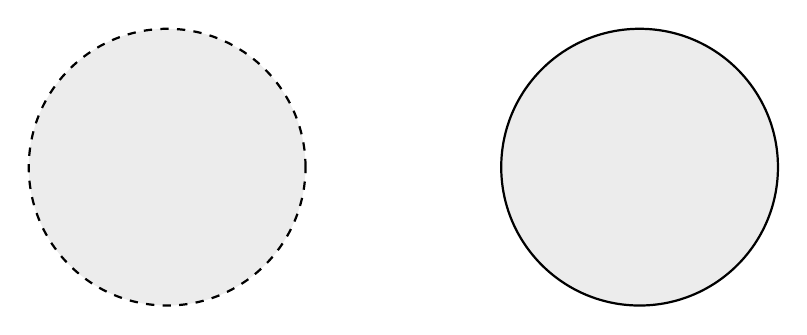
\begin{tikzpicture}
	\filldraw[color=black, fill=gray!15, thick, dashed] (0,0) circle (50pt);
	\filldraw[color=black, fill=gray!15, thick ] (6,0) circle (50pt);
	\end{tikzpicture}
	\caption{Open and closed balls in $ \R^2 $.}
\end{figure}  
\subsection{Open Sets, Closed Sets, and Boundaries}
We want to generalize the notion of open and closed balls in $ \R^n $ to any metric space. In order to do these, we'll need to outline a couple preliminary definitions that classify the elements of a metric space. 
\begin{definition}
	A \textit{\color{red}neighborhood } of $ x $ in a metric space $ X $ is defined as $ N_r(x)=\{y\in X\mid d(x,y)<r\} $ for a radius $ r>0 $.  
\end{definition}
As the name implies, a neighborhood centered at $ x $ is simply all the points ``around'' $ x $. A neighborhood is its own set, and we will use them constantly. They are sort of like ``sets of utility'', because we will use them as tools to analyze the properties of other sets. If there is a set $ E $ in a metric space $ X $, we can use neighborhoods in $ X $ to learn about the points in $ E $. Are some neighborhoods subsets of $ E $? Do some neighborhoods intersect $ E $? Will the answers to these questions change if we make $ r $ really big or really small? It is worth thinking about these questions taking $ E $ to be one of the balls defined in Definition 3.3. Do the answers change if $ E $ is an open ball versus a closed ball? 

 Much like the open ball of Definition 3.2, neighborhoods do not include the points that are exactly a distance of $ r $ away from the point $ x $. In fact, if our metric space is $ \R^n $ with the standard metric, a neighborhood and open ball are precisely the same. 
\begin{example}
	Let our metric space be $ \Z^2 $ equipped with the taxi-cab metric. Figure 10 shows the neighborhood centered at the origin of radius 3. 
		\begin{figure}[h]
		\centering
		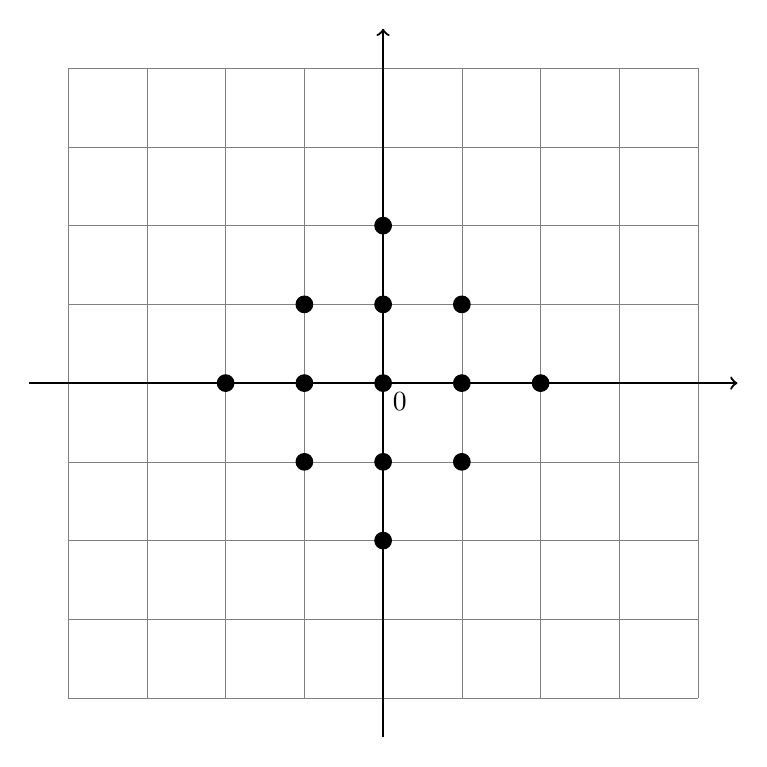
\begin{tikzpicture}
		\draw[step=1cm,gray,very thin] (-2,-2) grid (6,6);
		\draw[thick,->] (2,-2.5) -- (2,6.5);
		\draw[thick,->] (-2.5,2) -- (6.5,2);
		\filldraw (2,2) circle (3pt) node[anchor=north west] {$ 0 $};
		\filldraw (2,3) circle (3pt);
		\filldraw (2,4) circle (3pt);
		\filldraw (2,1) circle (3pt);
		\filldraw (2,0) circle (3pt);
		\filldraw (1,2) circle (3pt);
		\filldraw (1,3) circle (3pt);

		\filldraw (1,1) circle (3pt);
		
		\filldraw (0,2) circle (3pt);
		
		\filldraw (3,2) circle (3pt);
		\filldraw (3,3) circle (3pt);
		\filldraw (3,1) circle (3pt);
	
		\filldraw (4,2) circle (3pt);
	
	
		\end{tikzpicture}
		\caption{The set $ N_{3}(\mathbf{0})=\{\y\in\Z^2\mid|y_1|+|y_2|<3 \} $.}
	\end{figure}
\end{example} 
 
\begin{example}
Let $ d:\R^2\times\R^2\to[0,\infty] $ be the euclidean metric, and $ t:\R^2\times\R^2\to[0,\infty] $ be the taxi-cab metric. A neighborhood in $ (\R^2,d) $ may have a different ``shape'' then it would in $ (\R^2,t) $. We will denote $ N_{3}(\mathbf{0})\in \R^2 $ as $ E $ and $ F $, in $ (X,d) $ and $ (X,t) $ respectively. These neighboorhoods are shown in Figure 11.     
	\begin{figure}[h!]
	\centering
	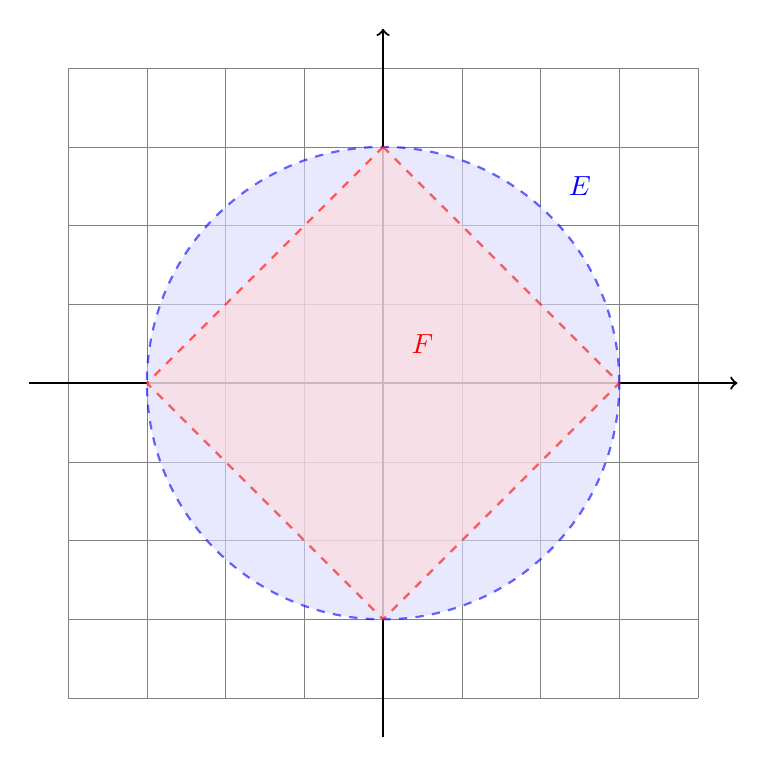
\begin{tikzpicture}
	\draw[step=1cm,gray,very thin] (-2,-2) grid (6,6);
	\draw[thick,->] (2,-2.5) -- (2,6.5);
	\draw[thick,->] (-2.5,2) -- (6.5,2);
	\filldraw[color=blue, fill=blue!15, thick, dashed, opacity=0.6] (2,2) circle (3cm);
	\filldraw[color=red, fill=red!15, thick, dashed, opacity=0.6] (2,5) -- (5,2) -- (2,-1) -- (-1,2) --(2,5) ;
	\draw[color = red] (2.5,2.5) node {$ F $};
	\draw[color = blue] (4.5,4.5) node {$ E $};
	\end{tikzpicture}
	\caption{$ N_{3}(\mathbf{0})\in \R^2 $ in $ (\R^2,d) $ and $ (\R^2,t) $. }
\end{figure}	
\end{example}
\begin{definition}
	Let $ X $ be a metric space. A point $ x\in X $ is a \textit{\color{red}limit point} of the set $ E\subset X $ if \textit{every} neighborhood of $ x $ contains a point $ y\in E $, where $ y\neq x $. We will denote the \textit{\color{red} set of all limit points} of $ E $ as $ E'=\{x\in X\mid x\text{ is a limit point of }E \}=\{x\in X\mid \in (N_r(x)\cap E)\backslash\{x\}\neq\emptyset\ \forall r>0\} $.
\end{definition}
\begin{note}
	For the remainder of Section 2, we will use $ X $ to denote a metric space, and $ E $ as some subset of $ X $. 
\end{note}
A limit point of a set is in some sense always ``close'' to points of the set. If $ x $ is a limit point of $ E\subset X $, then $ N_r(x) $ will always include points other than $ x $, no matter what we take $ r $ to be! We could make $ r $ smaller and smaller, but the set $ N_r(x) $ will never just be $ x $. In this sense, a limit point can always be ``approximated'' by elements in $ E $.  
\begin{remark}
Definition $ 3.5 $ never specifically said that a limit point of some set belongs to the set. As the next example shows, being a limit point has nothing to do with whether or not a point is included in the set in question. 	
\end{remark}
\begin{example}
$\R^2$ is a good starting place. Suppose we have a set $ E\subset \R $ that for the most part forms a rectangle. The ``border'' of the rectangle is no included in $ E $. Also note that $ E $ includes an ``isolated'' point $ z $ (see Figure 12). Let's consider three points in $ \R^2 $: $ x $, $ y $, and $ z $.  
		\begin{figure}[h]
	\centering
	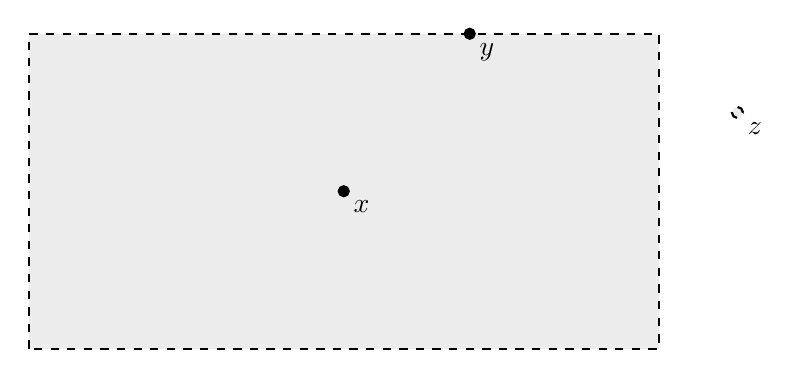
\begin{tikzpicture}
	\filldraw[color=black, fill=gray!15, thick, dashed] (0,0) rectangle (8,4);
	\filldraw (4,2) circle (2pt)node[anchor=north west] {$ x $};
	\filldraw (5.6,4) circle (2pt)node[anchor=north west] {$ y $};
	\filldraw[color=black, fill=gray!15, thick, dashed] (9,3) circle (2pt)node[anchor=north west] {$ z $};
	\end{tikzpicture}
	\caption{The set $ E\subset \R^2 $.}
\end{figure}

The point $ x $ belongs to $ E $. Furthermore, no matter what we take $ r $ to be, $ N_r(x) $ will never become a singleton of just $ \{x\} $. For the sake or argument, suppose $ x=(2,2) $. If $ r=0.5 $, then $ (2,2.49)\in N_{0.5}(x) $. Of $ r=0.01 $, then we still have $ (2,2.001)\in N_{0.01}(x) $. In fact, for every $ r $, we have $ (2,2+r/2)\in N_r(x) $. This means that $ x $ is a limit point of $ E $. 

Now consider $ y $. This point does not belong to $ E $, but it is still a limit point! We could repeat the same argument we made for $ x $ without running into trouble, because every neighborhood of $ y $ will include points ``just below'' $ y $, all of which are in $ E $! What matters with limit points is not what set the point belongs to, but what set the points nearby it belong to. 

Lastly, the point $ z $ is not a limit point. If we took $ r $ to be sufficiently large, then $ N_r(z) $ would include points in $ E $ that form the rectangle. Unfortunately, we could easily take $ r$ to be so small that $ N_r(z)=\{z\} $. It only takes one such $ r $ to rule out the chance of $ z $ being a limit point. We can provide a definition that corresponds to points like $ z $.     
\end{example}

\begin{definition}
		Let $ X $ be a metric space. For a set $ E\subset X $, $ x\in E $ is an \textit{\color{red}isolated point} if it is not a limit point. That is, there exists an $ r>0 $ such that $ N_r(x)=\{x\} $. 
\end{definition}
By the definition of an isolated point, it is the opposite of a limit point, rendering the two definitions mutually exclusive. This definition also means any point $ x\in X $ is \textit{either} a limit point \textit{or} an isolated point.  An isolated point of any set is also included in the set, which is not the case for limit points. 
\begin{definition}
Let $ X $ be a metric space. A point $ x\in X$ is an \textit{\color{red}interior point} of $ E\subset X $ if there exists \textit{a single} $ r>0 $ such that $ N_r(x)\subset E $. 
\end{definition}
\begin{example}
	Again, let's look at an example in $ \R^2 $. Let $ E\subset \R^2 $ be a closed ball that is ``punctured'' at $ z\in\R^2 $ such that $ z\notin E$. This can be seen in figure 13. The point $ x $ is in an interior point, as we could find some small $ r $ for which $ N_r(x)\subset E $. The point $ y $ is not an interior point of $ E $, because every single $ N_r(y) $ will contain some point outside of $ E $, meaning $ N_r(y)\not\subset E $. Finally, the point $ z $ is not an interior point, as each neighborhood of $ N_r(z) $ contains $ z $, and $ z\notin\ E $. Even though we can make $ r $ small enough to guarantee the only point in $ N_r(z) $ which is not in $ E $ is $ z $ $ (N_r(z)\backslash E=\{z\}) $, this point is all it takes to guarantee $ N_r(z)\not\subset E $ for all $ r $. 
\begin{figure}[h]
	\centering
	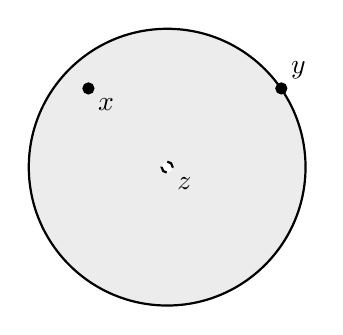
\begin{tikzpicture}
	
		\filldraw[color=black, fill=gray!15, thick ] (6,0) circle (50pt);
		\filldraw[color=black, fill=white, thick, dashed] (6,0) circle (2pt)node[anchor=north west] {$ z $};
		\filldraw (5,1) circle (2pt)node[anchor=north west] {$ x $};
		\filldraw (7.45,1) circle (2pt)node[anchor=south west] {$ y $};
	\end{tikzpicture}
	\caption{The set $ E\subset \R^2 $.}
\end{figure}	
\end{example}
\begin{remark}
	While a limit point of $ E\subset X $ need not be a point in $ E $, an interior point of $ E $ must be an element of $ E $. If $ x $ is an interior point, then $ x\in N_r(x)\subset E $ for some $ r $, so $ x\in E $. 
\end{remark}
\begin{example}
	It may be tempting to conclude that an interior point must be a limit point, after all, if we can find an $ N_r(x)\subset E $, then it is likely each neighborhood would contain infinite points of $ X $. This logic makes the dangerous assumption that $ X $ is in infinite, and $ d(x,y) $ ``behaves like'' the Euclidean metric. Consider a metric space $ X $ with the discrete metric $$ d(x,y)=\begin{cases}
	1\text{ if }x\neq y\\
	0\text{ if }x=y
	\end{cases}.$$ 
	For any $ x\in X $, $ N_{1/2}(x)=\{x\}\subset X $. We have that $ x $ is an interior point, but not a limit point. 
\end{example}
We now briefly introduce the idea of an exterior point. The only difference between the  definition of an interior point and exterior point, will be that the neighborhood of a point will be in the complement of $ E $ for an exterior point. This small change in language will make a big difference in meaning. 
\begin{definition}
Let $ X $ be a metric space. A point $ x\in X$ is an \textit{\color{red}exterior point} of $ E\subset X $ if there exists \textit{a single} $ r>0 $ such that $ N_r(x)\subset E^c $.
\end{definition}
\begin{remark}
Any point $ x\in X $ is \textit{either} an interior point \textit{or} an exterior point.
\end{remark}
\begin{example}
	Let $ [0,1]\in \R $. The point $ 2\in\R $ is an exterior point of $ [0,1] $. 
\end{example} 
\begin{remark}
	Nearly every definition in this section specifies a metric space $ X $. This means the metric space we work in could affect how we classify a point (and later sets). If we have two metric spaces $ X $ and $ Y $ where $ X\subset Y $, a point $ x\in E\subset X $ may be a limit point/interior point/exterior point in $ X $ but not in $ Y $. 
\end{remark}
\begin{example}
{\color{red}EXAMPLE }
\end{example}

We already generalized the idea of some open or closed interval in $ \R $ to the concept of an open or closed ball in $ \R^n $. Now we will go one step further, by bringing these concepts to any metric space. 
\begin{definition}
	Let $ X $ be a metric space. A set $ E\subset X $ is \textit{\color{red}open} if every point of $ E $ is an interior point.  
\end{definition}
\begin{definition}
	Let $ X $ be a metric space. A set $ E\subset X $ is \textit{\color{red}closed} if it contains all its limit points. That is, $ E'\subset E $. 
\end{definition}
\begin{example}
	Let $ (a,b)\subset\R $. This set is open, as for all $ x\in(a,b) $, we can find an $ r $ such that $ N_r(x)\subset(a,b) $. If $ d(a,x)\ge d(x,b) $, let $ r=d(x,b)/2 $. If $ d(x,b)>d(a,x) $ let $ r=d(x,a)/2 $.  Figure 14 shows this neighborhood for $ x $ where $ d(a,x)\ge d(b,x) $.
		\begin{figure}[h]
		\centering
		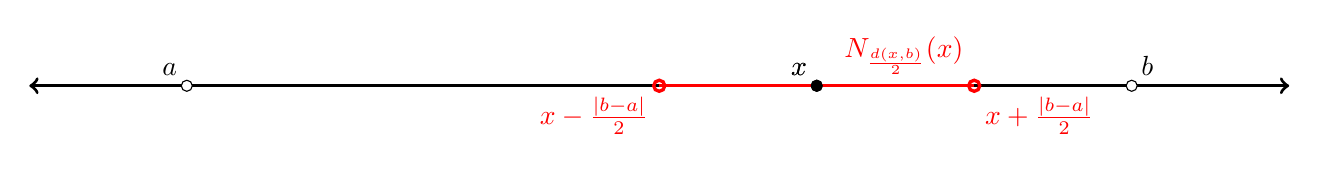
\begin{tikzpicture}
		\draw[very thick, color=red] (0,0) -- (2,0); 
		\draw[very thick, ->] (6,0) -- (8,0);
		\draw[very thick, ->] (-6,0) -- (-8,0);
		\draw[very thick] (-6,0) -- (6,0);
		\filldraw[fill=white] (-6,0) circle (2pt)node[anchor=south east] {$ a $};
		\filldraw[fill=white] (6,0) circle (2pt)node[anchor=south west] {$ b $};
		\filldraw[fill=black] (2,0) circle (2pt)node[anchor=south east] {$ x $};
		\draw[color=red, very thick] (4,0) circle (2pt)node[anchor=north west] {$ x+\frac{|b-a|}{2} $};
		\draw[color=red, very thick] (0,0) circle (2pt)node[anchor=north east] {$ x-\frac{|b-a|}{2} $};
		\draw[very thick, color=red] (0,0) -- (4,0) node[anchor=south east] {$ N_{\frac{d(x,b)}{2}}(x) $}; 
		\filldraw[fill=black] (2,0) circle (2pt)node[anchor=south east] {$ x $};
		\end{tikzpicture}
		\caption{The open interval $ (a,b)\subset \R $.}
	\end{figure}
By construction, our neighborhood will always be a proper subset of $ (a,b) $, so each point of $ x $ is an interior point. Therefore $ (a,b) $ is open. On the other hand, $ (a,b) $ is not closed, because $ a $ and $ b $ are limit points, but neither are in the set $ (a,b) $.
\end{example}
\begin{example}
	Let $ [a,b]\subset\R $. This set is not open, as $ a $ and $ b $ are not interior points. For instance, $ a-r/2\in N_r(a) $ for all $ r>0 $. The number $ a-r/2\notin[a,b] $, so $ N_r(a)\not\subset[a,b] $ for all $ r $. While $ [a,b] $ is not open, it is closed. Every point in $ [a,b] $ is a limit point because $ \R $ is complete. The interval $ [a,b] $ trivially contains itself, so it contains all its limit points and is closed. 
\end{example}
\begin{example}
Let $ X $ be a metric space, and $ E\subset X $. Any set with no limit points, $ E'=\emptyset $, is closed, because $ \emptyset\subset E $. This means any finite set is closed, as no finite set has limit points. Let $ X=\{x_1,\ldots, x_n\} $, and $ E\subset X $. If we let $ y\in E $, and set $ r=\min_{x\in X}d(x,y) $, then $ N_r(y)=\{y\} $. This means $ y $ fails to be a limit point for all $ y\in E $.
\end{example}
\begin{remark}
	The definitions of open and closed sets never imply that a set is either closed or open. It is possible for a set to be both closed and open, or be neither closed nor open.
\end{remark}
\begin{example}
The set $ \emptyset $ in any metric space $ X $ is closed and open. This set has no limit points $ (\emptyset'=\emptyset) $, and $ \emptyset\subset\emptyset $, so it is closed. The set also has no points, so every point is an interior point, making $ \emptyset $ open. 
\end{example}
\begin{example}
The set of rationals $ \Q $ is neither open nor closed in $ \R $. For all $ x\in\Q $, $ N_r(x) $ will contain irrational numbers for all $ r $, meaning $ N_r(x)\not\subset\Q $. Therefore no elements of $ \Q $ are interior points. The set $ \Q $ also does not contain all of its limit points, as any irrational number is a limit point as a result of Theorem 2.4. For example, any neighborhood of $ \sqrt{2} $ will contain elements of $ \Q $ (which are not $ \sqrt{2} $), making it a limit point. 
\end{example}
\begin{remark}
	The point made in Remark 3.3 is especially relevant for open and closed sets. A set could be open in one metric space, but closed in another. In most cases it's clear what metric space we are working in, but sometimes it is not. In cases where it is vague, it's always best to say a set is \textit{open in $ X $} or \textit{closed in $ X $}. For this reason it is a good practice to either specify $ E\subset X $, or include ``in $ X $.'' Many topics in analysis concern the metric space $ \R^n $ or $ \R $, so if you say a set is closed or open in conversation, it is usually assumed the metric space is one of these spaces. For example, if you were to ask someone ``are the integers closed or open?", they would most likely assume you mean ``are the integers closed or open in $ \R $?" 
\end{remark}

\begin{example}
	Suppose we want to determine if $ \Z $ is open or closed in $ \Z $. Every point is an interior point as $ N_{1/2}(x)={x}\subset\Z $ for all $ x\in\Z $, so $ \Z $ is open in $ \Z $. The set $ \Z $ has no limit points in $ \Z $, as $ N_{1/2}(x) $ does not include any points $ y\in\Z $ where $ y\neq x $. This gives that $ \Z'=\emptyset $,\footnote{This also means that every point of $ \Z $ is isolated.} so $ \Z\subset \Z' $, and $ \Z $ is closed in $ \Z $.
	
	 Now let our metric space be $ \R $. Is $ \Z $ open in $ \R $? Let $ x\in\Z $. For any $ N_r(x) $ such that $ r<1 $, $ x-r/2\in N_r(x) $, where $ x-r/2\notin\Z $. If $ r\ge 1 $, then $ x-1/2\in N_r(x) $, where $ x-1/2\notin\Z $.\footnote{The case where $ r\ge 1 $ handles the situation where $ r/2\in\Z $. If this were the case, then $ x-r/2\in\Z $. This is not a problem, as $ N_r(x) $ would still contain an uncountably infinite number of reals numbers, but it makes explicitly finding one of those reals a little tricky. It's easier to just add or subtract $ 1/2 $ from $ x $ and call it a day.} Therefore, there exists no $ r $ such that $ N_r(x)\subset \Z $, so $ \Z $ is not open in $ \R $. We have that $ \Z $ is closed in $ \R $, as each point of $ \Z $ is still isolated.  
\end{example}

Before proving some useful properties of open and closed sets, there is one more definition that can prove helpful at times. It formalizes the notion of points in a set that are just on the border of a set, like the endpoints of $ [a,b]\subset\R $.  
\begin{definition}
	Let $ X $ be a metric space, and $ E\subset X $. The \textit{\color{red}boundary} of $ E $, denoted $ \partial E $, is the set of points in $ X $ such that every neighborhood of $ p $ contains at least one point of $ E $ and at least one point not of $ E $. $$ \partial E=\{x\in X\mid N_r(x)\cap E\neq\emptyset\text{ and }N_r(x)\cap  E^c\neq\emptyset \ \forall r>0  \} $$ 
	Any element of $ \partial E $ is a \textit{\color{red}boundary point}.
\end{definition}
There are several equivalent definitions of $ \partial E $, many of which are more popular than this specific one. These other definitions use terms that we will cover in Section 3.4, so we will circle back then and discuss the boundary of a again. The first example one's mind should jump to are open and closed balls in $ \R^n $. 
  \begin{figure}[h]
  	\centering
  	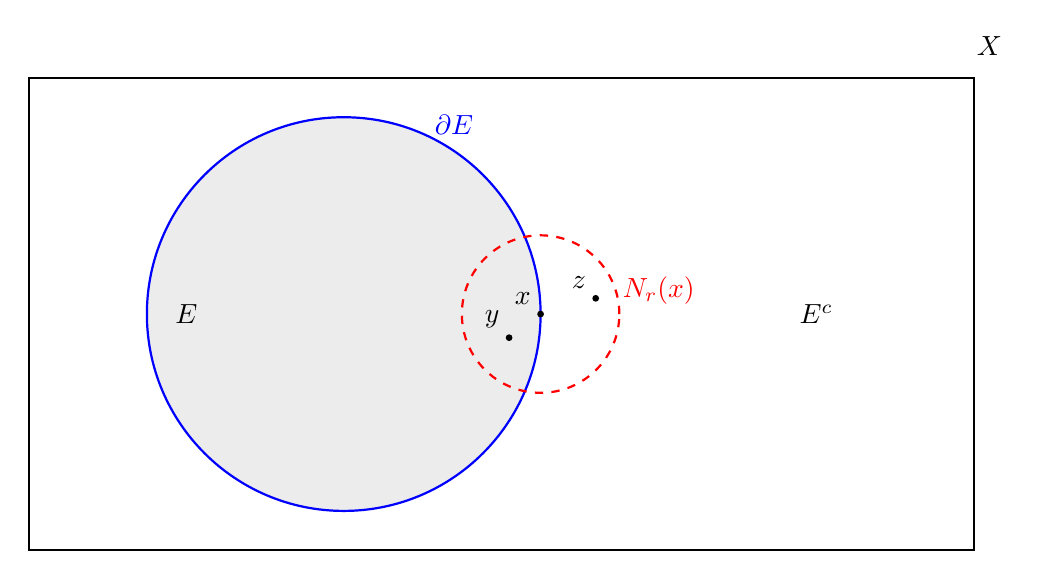
\begin{tikzpicture}
  	\draw[color=black, thick ] (0,0) rectangle (12,6);
  	\filldraw[color=blue, fill=gray!15, thick ] (4,3) circle (2.5cm);
  	\draw (12.2,6.4) node {$ X $};
  	\draw (2,3) node {$ E $};
  	\draw (10,3) node {$ E^c $};
  	\filldraw (6.1,2.7) circle (1pt) node[anchor = south east] {$ y $};
  	\filldraw (6.5,3) circle (1pt) node[anchor = south east] {$ x $};
  	\filldraw (7.2,3.2) circle (1pt) node[anchor = south east] {$ z $};
  	\draw[color=red,dashed, thick ] (6.5,3) circle (1cm);
  	\draw[color = red] (8,3.3) node {$ N_r(x) $};
  	\draw[color = blue] (5.4,5.4) node {$ \partial E $};
  	\end{tikzpicture}
  	\caption{The boundary of a set $ E $ is shown in blue. Let $ \x\in X $. No matter how small we make $ r $, $ N_r(x) $ will always contain some $ y\in E $ and some $ z\in E^c $, so $ x\in\partial E $. } 
  \end{figure}
\begin{example}
	Let $ B_r(\x) $ be the open ball of radius $ r $ centered at $ x\in\R^n $ (we could also denote this as $ N_r(\x) $). As the name suggests, the boundary is just all the points that are exactly a distance of $ r $ away from $ \x $, meaning $ \partial B_r(\x)=\{\y\in X\mid |\x-\y|=r\} $. In this particular case, no points in the boundary are in $ B_r(\x) $, so we have $ B_r(\x)\cap\partial B_r(\x)=\emptyset  $. If we take $ \bar{B}_r(\x) $ to be the closed ball, then we have the same boundary. $$\partial \bar{B}_r(\x)=\partial B_r(\x)=\{\y\in X\mid |\x-\y|=r\} $$ We also have $ \partial \bar{B}_r(\x)\cap \bar{B}_r(\x)=\bar{B}_r(\x)  $, and $ B_r(\x)\cup\partial B_r(\x)=\bar{B}_r(\x) $. 
\end{example}
\begin{remark}
	It is very tempting to think all boundary points are limit points. At first glance, the definition of a boundary point seems to imply a point $ x\in\partial E $ is not only a limit point of $ E $, but also a limit point of $ E^c $. This is not true! Suppose $ x\in E $ is a limit point. The definition of a limit point not only requires that $ N_r(x)\cap E $ for all $ r $, but also requires that there are points \textit{other than} $ x $ in $ N_r(x) $. A boundary point needn't satisfy this second requirement, so even if $ N_r(x)\cap E=\{x\} $ for all $ r $, $ x $ can still be a boundary point! 
\end{remark}

\begin{example}
	Let $ E\subset \R^2 $ be the union of a disk punctured at $ z $ and an isolated point $ y $ (Figure 16).  
	\begin{figure}[h]
		\centering
		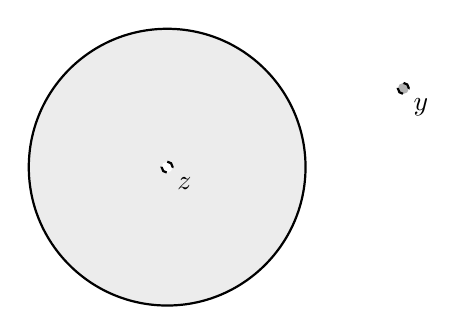
\begin{tikzpicture}
		\filldraw[color=black, fill=gray!15, thick ] (6,0) circle (50pt);
		\filldraw[color=black, fill=white, thick, dashed] (6,0) circle (2pt)node[anchor=north west] {$ z $};
		\filldraw[color=black, fill=gray!60, thick, dashed] (9,1) circle (2pt)node[anchor=north west] {$ y $};
		\end{tikzpicture}
		\caption{The set $ E\subset \R^2 $.}
	\end{figure}

The points $ y $ and $ z $ are both boundary points. Despite this, $ y $ is not a limit point of $ E $, and $ z $ is not a limit point of $ E^c $. This follows from the reasoning in the previous remark.  	
\end{example}

\begin{remark}
	We have now introduced five different definitions that classify points: limit points, isolated points, interior points, boundary points, and exterior points. This is \textit{a lot} to take in all at once. By far the most important concepts introduced here were open and closed sets. Being able to determine if a set is open and/or closed is one of the most important skills to have for this section, and those that follow. 
\end{remark}
\subsection{Properties of Open and Closed Sets}
Open set and closed sets will play a roll in many of the results and theorems to come, so it is important to be able to identify which sets are open and which are closed. We will know introduce several tools that make this easier.  
\begin{proposition}
	Every neighborhood is an open set.
\end{proposition}
\begin{proof}
	Suppose we have a metric space $ X $, and some point $ x\in X $. We will show that any point $ y\in N_r(x) $ is an interior point. There exists some $ h $ such that $$d(x,y)=r-h .$$ I claim that $ N_{r'}(y)\subset E $ for $ r'<h $. For all points $ z $ such that $ d(y,z)=r'<h $, the triangle inequality gives $$d(x,z)\le d(x,y)+d(y,z)<r-h+h=r, $$ so $ z\in N_r(x)=E $ for all $ z $ by the definition of $ N_r(x) $. This implies that $ N_{r'}(y)\subset E $, making $ y $ an interior point. (Figure 17)
	\begin{figure}[h]
		\centering
		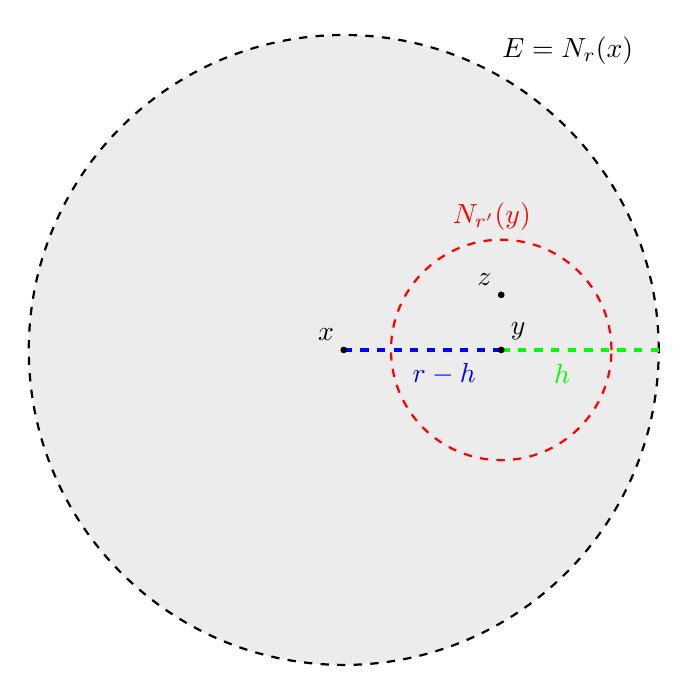
\begin{tikzpicture}
		\filldraw[color=black, fill=gray!15, thick, dashed ] (6,0) circle (4cm);
		\draw[very thick, dashed, color=blue] (6,0) -- (8,0);
		\draw[color=blue] (7.8,-0.3) node[anchor = east] {$ r-h $};
		\draw[very thick, dashed, color=green] (8,0) -- (10,0);
		\draw[color=green] (9,-0.3) node[anchor = east] {$ h $};
		\draw[color=black] (9.8,3.8) node[anchor = east] {$ E=N_r(x)$};
		\filldraw (6,0) circle (1pt) node[anchor = south east] {$ x $};
		\filldraw (8,0) circle (1pt) node[anchor = south west] {$ y $};
		\filldraw (8,0.7) circle (1pt) node[anchor = south east] {$ z $}; 
		\draw[color=red] (8.5,1.4)  node[anchor = south east] {$ N_{r'}(y) $};
		\draw[color=red, thick, dashed] (8,0) circle (1.4cm); 
		\end{tikzpicture}
		\caption{The set $ E\subset X $. We constructed a neighborhood $ N_{r'}(y) $ for an arbitrary $ y\in N_r(x) $ such that $ N_{r'}(y)\subset E $. }
	\end{figure}
\end{proof}

\begin{proposition}
	If $ x\in X $ is a limit point of $ E $ ($ x\in E' $), then every neighborhood of $ x $ contains infinitely many points of $ E $.
\end{proposition}
\begin{proof}
	Let $ x\in X $. Suppose for contradiction, there exists some $ N_r(x) $ which contains only a finite number of points of $ E $. Let this finite set of points be $ \{y_1, \ldots, y_n\}\subset N_r(x)\cap E $. Pick the radius of $ N_r(x) $ to be the distance between $ x $ and the point to which it is closest in the finite set $ \{y_1,\ldots,y_n\} $: $$ r=\min_{1\le m\le n} d(x,y_m). $$ By construction, $ N_r(x) $ contains no point $ y\in E $ such that $ y\neq x $, so $ x $ is not a limit point of $ E $. This is a contradiction. (Figure 18)
	\begin{figure}[h]
		\centering
		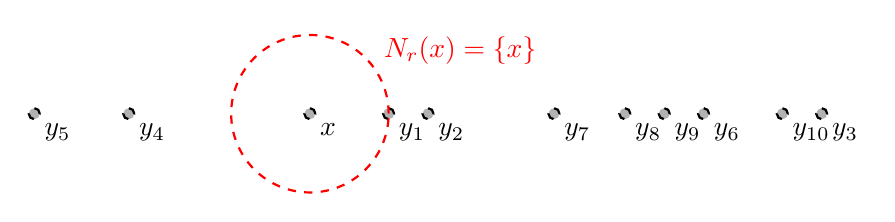
\begin{tikzpicture}
		\filldraw[color=black, fill=gray!60, thick, dashed] (1,0) circle (2pt)node[anchor=north west] {$ y_1 $};
		\filldraw[color=black, fill=gray!60, thick, dashed] (0,0) circle (2pt)node[anchor=north west] {$ x $};
		
		\filldraw[color=black, fill=gray!60, thick, dashed] (1.5,0) circle (2pt)node[anchor=north west] {$ y_2 $};
		\filldraw[color=black, fill=gray!60, thick, dashed] (6.5,0) circle (2pt)node[anchor=north west] {$ y_3 $};
		\filldraw[color=black, fill=gray!60, thick, dashed] (-2.3,0) circle (2pt)node[anchor=north west] {$ y_4 $};
		\filldraw[color=black, fill=gray!60, thick, dashed] (-3.5,0) circle (2pt)node[anchor=north west] {$ y_5 $};
		\filldraw[color=black, fill=gray!60, thick, dashed] (5,0) circle (2pt)node[anchor=north west] {$ y_6 $};
		\filldraw[color=black, fill=gray!60, thick, dashed] (3.1,0) circle (2pt)node[anchor=north west] {$ y_7 $};
		\filldraw[color=black, fill=gray!60, thick, dashed] (4,0) circle (2pt)node[anchor=north west] {$ y_8 $};
		\filldraw[color=black, fill=gray!60, thick, dashed] (4.5,0) circle (2pt)node[anchor=north west] {$ y_9 $};
		\filldraw[color=black, fill=gray!60, thick, dashed] (6,0) circle (2pt)node[anchor=north west] {$ y_{10} $};
		\draw[color=red, thick, dashed] (0,0) circle (1cm);
		\draw[color=red] (3,.5)  node[anchor = south east] {$ N_{r}(x)=\{x\} $};
		\end{tikzpicture}
		\caption{If our finite set of points of $ E $ is $ \{y_1,\ldots,y_{10}\} $, then we can reach a contradiction by constructing a neighborhood of $ x $ with $ r=\min_{1\le m\le n} d(x,y_m)=d(x,y_1) $. This will hold no matter where the points  $ \{y_1,\ldots,y_{10}\} $ happen to be in $ E $. In this case $ x\in E $, but remember that this isn't a requirement.}
	\end{figure}
\end{proof}
	
\begin{corollary}
A finite set has no limit points. (see Example 3.13)
\end{corollary}
The next theorem and its corollary allows us to determine if a set is open or closed based on its complement. At first, this may not seem helpful, but if it is not clear if $ E $ is open or closed, one can just use $ E^c $! We will provide examples where using $ E^c $ is easier.
\begin{theorem}
	A set $ E $ is open \textit{if and only if} its complement is closed.
\end{theorem}
\begin{proof}{\color{white}space}
	\begin{enumerate}
		\item [$ (\Longrightarrow) $] Suppose $ E $ is open. Let $ x\in X $ be a limit point of $ E^c $. Every neighborhood $ N_r(x) $ contains a point of $ E^c $, so $ N_r(x)\not\subset E $, meaning $ x $ is \textit{not} and interior point of $ E $. But we have assumed every point of $ E $ is an interior point, so $ x\in E^c $. Therefore $ E^c $ includes all its limit points and is closed.   
		\item [$ (\Longleftarrow) $] Suppose $ E^c $ is closed. Let $ x\in E $. We have $ x\notin E^c $, so $ x $ is not a limit point of $ E^c $ (otherwise it would be in $ E^c $, as $ E^c $ is closed). If $ x $ is not a limit point of, then there exists an $ N_r(x)\cap E^c=\emptyset $, giving $ N_r(x)\subset E $. Thus $ x\in E $ is an interior point, and $ E $ is open.  
	\end{enumerate}
\end{proof}
\begin{corollary}
	A set $ E $ is closed \textit{if and only if} its complement is open.
\end{corollary}
One practical consequence of these results, is that if you find it more difficult to check if a set is open or closed (or vice versa), you can always just work with the complement. 

\begin{example}
Let $ X $ be any metric space. Recall from Example 3.14 that $ \emptyset $ is closed and open. This means that $ \emptyset^c=X $ is closed and open as well. This allows us to conclude that $ \R $ in $ \R $ is open and closed.
\end{example}
\begin{example}
	The set $ [a,b]\subset \R $ is closed. This implies that $ [a,b]^c=(-\infty,a)\cup(b,\infty) $ is open.
\end{example}
We often define some set of interest as a union or intersection of a collection of sets. For instance, the proof of Theorem 1.2, the supremum of a set in $ \R $ was defined as the union of the Dedekind cuts that comprise the set. In Example 1.26, $ \Q $ was written as the countably infinite union of intervals. In situations like this, it is possible to know if a set is open or closed if the sets over which we take the union/intersection are open or closed. 
\begin{theorem}
	Let $ \{G_\alpha\} $ and $ \{F_\alpha\} $ be an arbitrary collection of open sets and closed sets respectively. Let $ G_1,\ldots,G_n $ and $ F_1,\ldots, F_n $ be a finite collection of open sets and closed sets respectively. In this case we have:
	\begin{enumerate}
		\item $ \bigcup_\alpha G_\alpha $ is open.
		\item $ \bigcap_\alpha F_\alpha $ is closed.
		\item $ \bigcap_{i=1}^n G_i$ is open.
		\item $ \bigcup_{i=1}^n F_i$ is closed.
	\end{enumerate}

\end{theorem}

\begin{proof}{\color{white}space}
	\begin{enumerate}
		\item Suppose $ G_\alpha $ is open for all $ \alpha $. Let $ x\in \bigcup_\alpha G_\alpha $. For some $ \alpha $, $ x\in G_\alpha $. There exists a neighborhood $ N_r(x) $ such that $ N_r(x)\subset G_\alpha $, because $ G_\alpha $ is open. Therefore $ \bigcup_\alpha G_\alpha $ is open, as $ N_r(x)\subset G_\alpha\subset \bigcup_\alpha G_\alpha $. 
		\item Suppose $ F_\alpha $ is closed for all $ \alpha $. It suffices to show that $ (\bigcap_\alpha F_\alpha)^c $ is open using Theorem 2.1. By the aforementioned theorem, $ F_\alpha^c $ is closed for all $ \alpha $. Therefore the union of $ F_\alpha^c $ is open by part (1). This completes our proof, as De Morgan's Law gives $$ \left(\bigcap_\alpha F_\alpha\right)^c=\bigcap_\alpha F_\alpha^c.$$
		\item Suppose the sets $ G_1,\ldots,G_n $ are open. Let $ x\in \bigcap_{i=1}^n G_i$. For all $ x\in\bigcap_{i=1}^n G_i $, there exists neighborhoods $ N_{r_i}(x) $ with radii $ r_i $, such that $ N_{r_i}(x)\subset G_i $ for all $ i $. Let $ r=\min\{r_1,\ldots,r_n\} $. This radius gives us $ N_r(x)\subset G_i $ for all $ i $, meaning $ N_r(x)\subset \bigcap_{i=1}^n G_i $. Therefore $ x $ is an interior point, and $ \bigcap_{i=1}^n G_i $ is open. (Figure 19)   
		\begin{figure}[h!]
			\centering
			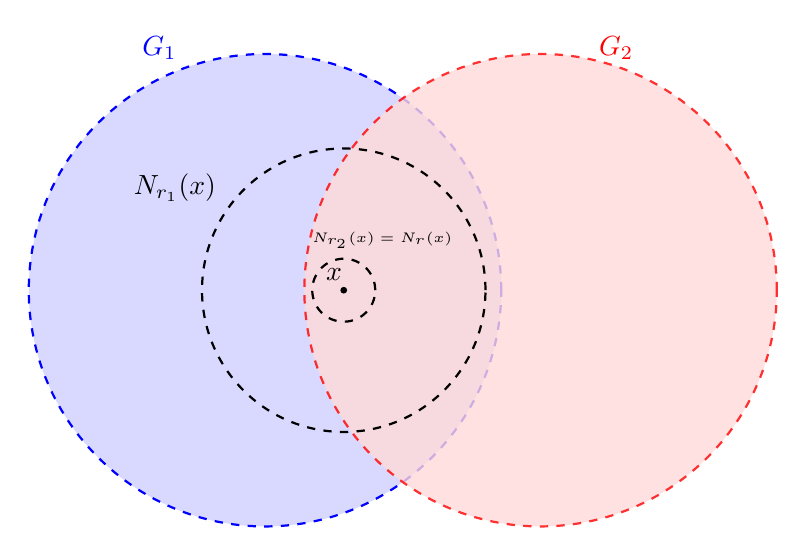
\begin{tikzpicture}
				\filldraw[color=blue, fill=blue!15, thick, dashed, opacity=1] (0,0) circle (3cm);\filldraw[color=red, fill=red!15, thick, dashed, opacity=0.8] (3.5,0) circle (3cm);
				\draw[color=blue] (-1,2.8)  node[anchor = south east] {$ G_1 $};
				\draw[color=red] (4.8,2.8)  node[anchor = south east] {$ G_2 $};
				\filldraw(1,0)  circle (1pt);
				\draw (1.1,0) node[anchor = south east] {$ x $};
				\draw[dashed, thick] (1,0) circle (1.8cm);
				\draw[dashed, thick] (1,0) circle (0.4cm);
				\draw(-0.5,1)  node[anchor = south east] {$ N_{r_1}(x) $};
				\draw(2.5,0.4)  node[anchor = south east] {\tiny$ N_{r_2}(x)=N_r(x) $};
			\end{tikzpicture}
			\caption{In this simplified setting, we have two open sets: $ G_1 $, and $ G_2 $. By letting $ r=\min\{r_1,r_2\}=r_2 $, we find a neighborhood $ N_r(x) $ such that $ N_r(x)\subset G_1\cap G_2 $. }
		\end{figure}
		\item  Suppose the sets $ F_1,\ldots,F_n $ are closed. It suffices to show that $ (\bigcap_{i=1}^n F_i)^c $ is open using Theorem 2.1. By the aforementioned theorem, $ F_i^c $ is open for all $ i$. By part (2) the the intersection of all $ F_i^c $ is open This complete out proof, as De Morgan's Law gives 
		 $$ \left(\bigcap_{i=1}^n F_i\right)^c=\bigcap_{i=1}^n F_n^c.$$
	\end{enumerate}
\end{proof}
Part (2) and (4) of Theorem 2.2 require that the collection of sets is finite, otherwise the minimum over the finite number of radii of neighborhoods many not be well defined. The following two examples show that Theorem 2.2 does not hold if we take these collections to be infinite. 
\begin{example}
	Let $ G_n=(1/n,1+1/n) $ for all $ n\in\N $. The set $ G_n $ is open in $ \R $ for all $ n $. Taking the intersection gives $$\bigcap_n G_n=[0,1] .$$ The interval $ [0,1] $ is closed, despite each $ G_n $ being open.  
\end{example}
\begin{example}
	Let $ F_n=[1/n,\infty) $ for all $ n\in\N $. The set $ F_n $ is closed in $ \R $ for all $ n $. Taking the union gives $$ \bigcup_{n}F_n=(0,\infty).$$ This interval is open in $ \R $, despited each $ F_n $ being closed.
\end{example}
\subsection{Closures, Interiors, Dense Sets, and Perfect Sets} 
There are a handful of other definitions related to open set and closed sets that deserve a bit of attention.
\begin{definition}
Let $ X $ be a metric space. The \textit{\color{red}interior} of a set $ E\subset X $, denoted $ E^\circ $, is the set of all interior points of $ E $. $$ E^\circ=\{x\in X\mid x\text{ is an interior point of }E \} $$
\end{definition}
The set $ E^\circ $ is clearly open, as by definition it is comprised only of interior points. Because interior points of $ E $ must be in $ E $, we have $ E^\circ \subset E $. Informally, we can think of $ E^\circ $ as the smallest open set contained within $ E $. This interpretation leads to the conclusion that if $ E $ is open, then $ E=E^\circ $.
\begin{example}
	Let $ [a,b]\subset\R $. The interior of this set is $ (a,b) $. 
\end{example}
\begin{definition}
	Let $ X $ be a metric space. The \textit{\color{red}closure} of a set $ E\subset X $ is $ \bar{E}=E\cup E' $. 
\end{definition}
The closure $ \bar{E} $ is the opposite of the interior in a certain sense. The closure can be though of as the smallest closed set that $ E $ is contained in. If $ E $ is closed, then $ E'\subset E $, and $ E=\bar{E} $.
\begin{example}
	Let $ (a,b)\subset\R $. The closure of this set is $ [a,b] $. 
\end{example}
\begin{definition}
	Let $ X $ be a metric space. The set $ E\subset X $ is \textit{\color{red}dense in $ X $} if every point of $ X $ is a limit point of $ E $, or a point of $ E $. ($ \bar{E}=X $)  
\end{definition}

Informally, if $ E $ is dense in $ X $, then we can approximate any point of $ X $ with a point in $ E $ arbitrarily well. This follow from the fact that any point in $ X $ is either in $ E $, or a limit point of $ E' $, or both.  We have already seen one example of this with Theorem 1.4.
\begin{example}
	The set $ \Q $ is dense in $ \R $, that is $ \bar{\Q}=\R $. One implication of this fact is that the irrational numbers $ \R\backslash\Q $ are limit points of $ \Q $. 
\end{example}
Many results involving approximation can be stated in terms of dense sets. One of these is the Weierstrass Approximation Theorem. This will be formally treated and proved in Section 7, but for now we will give the result as an example of a dense set.
\begin{example}[Weierstrass Approximation Theorem]
	Let $ \mathscr{C}([a,b])=\{f\mid f:[a,b]\to \R\text{ and } f\text{ continuous}\} $ be the set of real valued continuous functions with domain $ [a,b] $. Now let $ \mathscr{P}([a,b]) $ be the set of all real valued polynomials with domain $ [a,b] $.\footnote{This set is traditionally denoted as $ \R[x] $ in abstract algebra.} The set $ \mathscr{P}([a,b])  $ is dense in $ \mathscr{C}([a,b]) $. We will always be able to approximate a continuous function on a bounded interval arbitrarily well with polynomials. This result, and spaces of functions, will be discussed again in Section 7. 
\end{example}
\begin{definition}
	Let $ X $ be a metric space. The set $ E\subset X $ is \textit{\color{red}perfect} if every point of $ E $ is a limit point of $ E $ $ (E=E') $. 
\end{definition}
If $ E $ is perfect, every point in $ E $ can be approximated arbitrarily well by other points in $ E $. 
\begin{example}
	The real line $ \R $ is a perfect set. 
\end{example}
\subsection{Compact Sets}
We have encountered infinity several times now. Sets can have an infinite number of element, in which case they are either countable or uncountable. A set can ``take up an infinite amount of space'' if it is unbounded. Each limit point of a set contains an infinite number of points in the set. These factors can result in sets that are difficult to work with. For example, suppose a set is unbounded. It can be hard to determine how functions or sequences behave on sets like this, because the distance between points can become arbitrarily large. What kind of headaches to limit points cause? Any neighborhood of a limit point will contain an infinite number of points in that set (Proposition 2.2). If the limit point is not in the set, this can also pose problems. As we will see later on, it could be possibly to get arbitrarily close to that limit point while never leaving the set. In a sense, we would be getting closer to a point in a set, where the destination is not even included in the set. To prevent this from happening, all limit points should be included in a set, i.e the set should be closed. Later on when working with sequences and continuous functions, two concepts intrinsically linked by the idea of getting arbitrarily close to a point, sets that are ``nice'', and will not illicit the two mentioned complications, will lead to nice results. Our goal now is to characterize these sets, and attempt to motivate their characterization.\footnote{Motivating the main definition of this subsection is infamously difficult, as it is not clear how it will be used in the future. It would be like explaining what a hammer is to someone who has no idea what a nail is. }   

One somewhat trivial way to guarantee a set is both closed and bounded is by restricting out attention to finite sets. If $ E $ is finite, it has no limit points and is trivially closed. A finite set must also be bounded. While finite may have the nice properties we are looking for, they are not that interesting. Real analysis almost always involves the real numbers, an uncountably infinite set. So what criteria would guarentee an infinite set, whether it be countable or uncountable, will behave like a finite set?

The way we will go about defining these sets is by looking how we can ``cover'' them with a collection of open sets. The idea is that a set may be infinite, but perhaps we can cover it with a finite collection of open sets. 
\begin{definition}
	Let $ X $ be a metric space. An \textit{\color{red}open cover} of a set $ E\subset X $ is a collection of open sets $ \mathcal\{G_\alpha\}\subset X $ such that $ E\subset\cup_\alpha G_\alpha $.  
\end{definition}
  \begin{figure}[h]
	\centering
	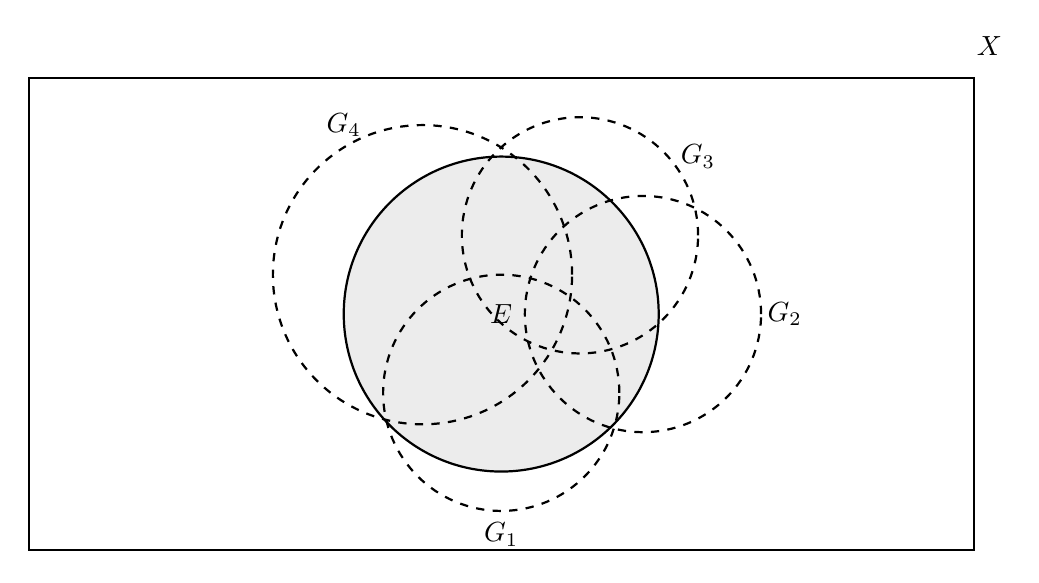
\begin{tikzpicture}
	\draw[color=black, thick] (0,0) rectangle (12,6);
	\filldraw[thick, fill=gray!15] (6,3) circle (2cm);
	\draw (12.2,6.4) node {$ X $};
	\draw (6,3) node {$ E $};
	\draw[thick, dashed] (6,2) circle (1.5cm);
	\draw (6,0.2) node {$ G_1 $};
	\draw[thick, dashed] (7.8,3) circle (1.5cm);
	\draw (9.6,3) node {$ G_2 $};
	\draw (8.5,5) node {$ G_3 $};
	\draw (4,5.4) node {$ G_4$};
	\draw[thick, dashed] (7,4) circle (1.5cm);
	\draw[thick, dashed] (5,3.5) circle (1.9cm);
	\end{tikzpicture}
	\caption{The collection of set $ \{G_1,\ldots G_4\} $ forms an open cover of $ E $.} 
\end{figure}
An open cover is a \textit{collection} of sets. Each element of an open cover is a single open set. This means that the cardinality of an open set has \textit{nothing} to do with the cardinality of the sets it is comprised of. The collection $ \{\R,(0,1),(0,2)\} $ is 3. We do not care whatsoever about the fact that each of the sets in the collection are uncountably infinite. The emphasis here is due to the fact that the cardinality of these covers (and a second type we will define soon) will be the bases of our criteria of what makes a set ``nice''.
\begin{example}
	Let $ E=N_r(x) $ be a subset of a metric space $ X $. One open cover of the set $ E $ is the single set $ N_{r+1}(x) $. Another would be $ N_{r+2}(x) $. 
\end{example}
\begin{example}
	Let $ \R $ be the entire real line. We can cover this with the union of all sets of the form $G_n=(-n,n)$ for $ n\in\N $. $$ \R\subset\bigcup_{n\in \N}(-n,n)$$
\end{example}
It is not enough to require that a set has a finite open cover. Any set $ E $ can trivially be covered by itself, forming an open cover consisting of one element. We could require that every open cover is finite, but this could never be satisfied. For example, take the closed interval $ (a,b)\subset\R $. We could cover this with a finite open cover $ \{(a,b)\} $. We could also cover it with the infinite open cover $ \{(a,b),(-1,1),(-2,2),(-3,3),\ldots\} $. We can just take the cover $ \{(a,b)\} $ and throw in an infinite number of random intervals of $ \R $ and still end up with an open cover. This is complete ``overkill'' when it comes to covering $ (a,b) $! To address the fact that we will always have infinite open covers, we will introduce a new type of open cover that is both finite, and limits any redundant additions to the cover. 

\begin{definition}
Let $ X $ be a metric space, and $ E\subset X $. A \textit{\color{red}finite subcover} of an open cover $ \{G_\alpha\} $ of $ E $  is a collection of open sets $ \{G_{\alpha_1},\ldots,G_{\alpha_n}\} $ such that $$ E\subset \bigcup_{i=1}^nG_{\alpha_i}\subset\bigcup_\alpha G_\alpha. $$
\end{definition}
\begin{example}
	Let $ X $ be a metric space and $ E\subset X $. The collection $ \{E\} $ is a trivial open cover. We also have a trivial finite open subcover in $ \{E\} $. 
\end{example}
\begin{example}
	Let $ \{(a,b),(-1,1),(-2,2),(-3,3),\ldots\} $ be an open cover of $ (a,b)\subset \R $. One finite subcover of this open cover is $ \{(a,b)\} $. Another finite subcover is $ \{(a,b),(-1,1)\} $. In fact, any set $ \{(a,b),(-1,1),\ldots(-n,n)\} $ is a finite subcover. 
\end{example}
This simple example shows that some open covers actually have an infinite number of finite subcovers. The introduction of finite subcovers may be a bit confusing, so it is worth recapping what we have done before presenting the main definition of this subsection: 
\begin{itemize}
	\item We have some metric space $ X $ and some set $ E\subset X $. We can cover this set with a collection of sets $ \{G_\alpha\} $ called an open cover, the cardinality of which is determined by the number of sets in the collection $ \{G_\alpha\} $. We like the idea of finite open covers.
	\item There exists an infinite number of open covers of a set. There also always exists a finite open cover of a set, so we need to do better than just having a finite open cover.  
	\item A finite subcover $ \{G_{\alpha_1},\ldots,G_{\alpha_n}\} $ of the open cover $ \{G_\alpha\} $ is a subset of $ \{G_\alpha\} $, which also covers $ E $. The finite subcover of one open cover $ \{G_\alpha\} $ \textit{is not necessarily} a finite subcover of another open cover $ \{G'_\alpha\} $, so whenever we talk about finite subcovers, it is with respect to some fixed open cover. Some open covers of sets have an infinite number of finite subcovers (Example 2.29).
\end{itemize} 
We are now ready give a proper definition and name to the ``nice'' sets we want to characterize. In doing so, we will answer an important question about finite subcovers that may have arisen by now -- some open covers of sets have an infinite number of finite subcovers, but do \textit{all} open covers of a set have \textit{at least one} finite subcover? 
\begin{definition}
	Let $ X $ be a metric space, and $ K $ be a subset of $ X $. The set $ K $ is \textit{\color{red}compact} if \textit{every} open cover of $ K $ contains \textit{at least one} finite subcover. 
\end{definition} 
The answer to our question turns out to be no. If it were yes, then there would be no need to define compactness, because every set would be compact. Compact sets turn out to be the nice sets we were looking for. As we'll see, they can be infinite, but they do not cause the complications with infinity that we discussed at the open of this subsection. In some sense, compact sets are the next best thing to finite sets. 
\begin{example}
	The set $ (a,b)\subset\R $ is not compact. In order verify this, we just need to find a single open cover that has no finite subcover. Let $ \{G_n\} $ be an open cover where $ G_n=(a+1/n,b) $. We have that $$ (a,b)\subset\bigcup_{n\in \N} G_n=\bigcup_{n\in \N}(a+1/n,b)=(a,b).$$ No finite subset of $ \{G_n\} $ will be a finite subcover of $ (a,b) $. If we had a finite subset of $ \{G_n\} $ then there would exist some $ N\in\N $ such that $ (a,a+1/N) $ is ``uncovered''. Therefore any open interval in $ \R $ is not compact. 
\end{example}
\begin{example}
	The real line $ \R $ is not compact. The open cover $ \{G_n\} $ where $ G_n=(-n,n) $ has no finite subcover. If we had a finite subset of $ \{G_n\} $, then there would exist some $ N\in\N $ such that $ (-\infty,-N)\cup(N,\infty) $ is ``uncovered''. Therefore the real line $ \R $ is not compact. 
\end{example}

These two examples should not be entirely surprising. When compactness was motivated, complications involving two types of sets were cited: unbounded sets, and sets that were not closed. $ (a,b) $ and $ \R $ both fall into exactly one of these categories.
\begin{example}
	Suppose $ X=\{x_1,\ldots,x_n\} $ is a finite metric space. The entire space $ X $ is compact. Let $ \{G_\alpha\} $ be an open cover of $ X $. For each $ x_i\in X $, there exists an $ G_{\alpha_i} $ such that $ x_i\in G_{\alpha_i} $. Therefore, the open cover has a finite subcover in $ \{G_{\alpha_1},\ldots ,G_{\alpha_n}\} $.    
\end{example}
Using the definition of compactness to verify that a set is not compact takes some creativity, but only requires one to find a single counterexample. This is opposed to verifying a set is compact. This requires we somehow verify that every single open cover has a finite subcover. This is prohibitively difficult to do in most cases. This is why we want to find conditions that are easy to verify and that imply compactness. Of chief concern, is doing this for subsets of $ \R^n $. 
\subsection{Properties of Compact Sets}
Before restricting our attention to $ \R^n $, we need to establish some properties of compact sets that will allow come in handy when working with them. Unfortunately, we still do not have any nontrivial examples of compact sets, so some of these results will not have examples presented alongside them. Once we are able to identify compact sets in $ \R^n $ by means other then the definition of compactness, these results can be verified. 
\begin{lemma}
	Suppose $ Y\subset X $. A subset $ E\subset Y$ is open in $ Y $ \textit{if and only if} $ E=Y\cap G $ for some open $ G\subset X $. 
\end{lemma}
\begin{proof}{\color{white}space}
	\begin{enumerate}
		\item[$ (\Longrightarrow) $] Suppose $ E\subset Y $ is open in $ Y $. For each $ x\in E $, there exists a $ r_x $ such that $ N_{r_x}(x)\subset E $. By the definition of a neighborhood, for all $ y\in Y $ satisfying $ d(x,y)<r_x $, we have $ y\in E $. Denote $ N_{r_x}(x)=V_x $ for all $ x\in E $, and define $$G=\bigcup_{x\in E}V_x .$$ The set $ G $ is a union of open sets, so it is open (Figure 21). I now claim that $ E=G\cap Y $, which is our desired result. For $ x\in E $, we have $ x\in V_x $ for all $ x\in X $, so $ x\in E $ and $ x\in Y $. This gives $ E\subset G\cap Y $. Now let $ x\in G\cap Y $. For the corresponding $ V_x $, $ V_x\cap Y\subset E $. This implies $ G\cap Y\subset E $.    
		\item[$ (\Longleftarrow) $] Suppose $ E=Y\cap G $ for some open $ G $ in $ X $. The set $ G $ is open, so for all $ x\in E $ there exists a neighborhood $ N_r(x)\subset E $. This gives $ N_r(x)\subset G $, as $ E=Y\cap G\subset G $. Intersecting $ N_r(x) $ with $ Y $ yields $ N_r(x)\cap Y\subset E $, so $ E $ is open in $ Y $.  
	\end{enumerate}	
 \begin{figure}[h!]
	\centering
	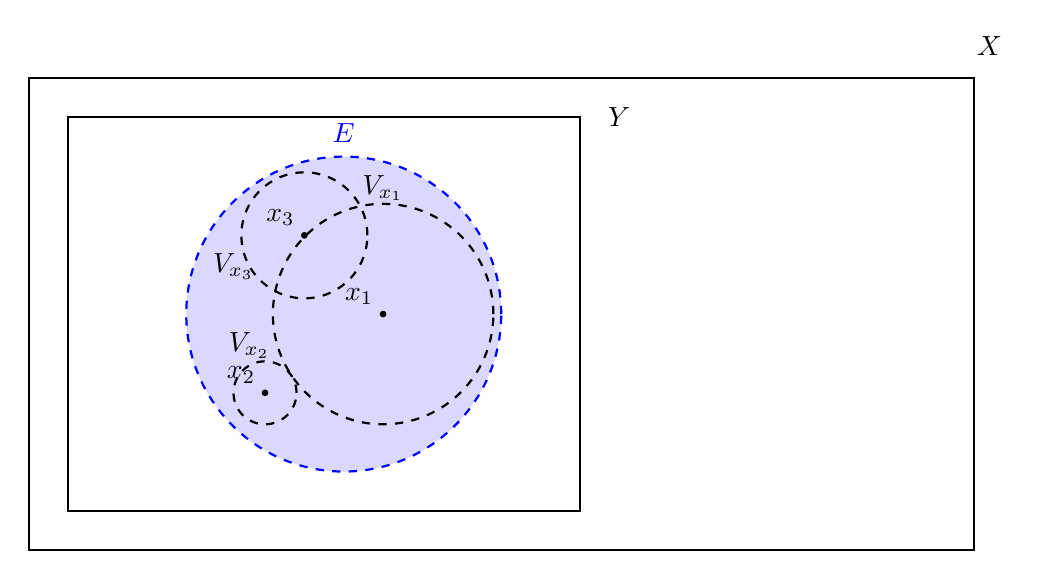
\begin{tikzpicture}
	\draw[color=black, thick] (0,0) rectangle (12,6);
	\draw[color=black, thick] (0.5,0.5) rectangle (7,5.5);
	\draw[black] (7.5,5.5) node {$ Y $};
	\draw (12.2,6.4) node {$ X $};
	\filldraw[color=blue, thick, dashed, fill=blue!15]  (4,3) circle (2cm);
	\draw[blue] (4,5.3) node {$ E $};
	\draw[thick, dashed]  (4.5,3) circle (1.4cm);
	\filldraw (4.5,3) circle (1pt) node[anchor= south east] {${x_1}  $}; 
	\draw (4.5,4.6) node {$V_{x_1} $};
	
	\draw[thick, dashed]  (3,2) circle (.4cm);
	\filldraw (3,2) circle (1pt) node[anchor= south east] {${x_2}  $}; 
	\draw (2.8,2.6) node {$V_{x_2} $};
		\draw[thick, dashed]  (3.5,4) circle (.8cm);
	\filldraw (3.5,4) circle (1pt) node[anchor= south east] {${x_3}  $}; 
	\draw (2.6,3.6) node {$V_{x_3} $};

	\end{tikzpicture}
	\caption{We take $ V_x $ to be the neighborhood of $ x $ contained in $ E $. We will always be able to find such a neighborhood because $ E $ is open in $ Y $. In this case, we have shown only three such neighborhoods. The (possibly infinite) union of all such neighborhoods is $ G $, which itself is open.}  
\end{figure}
\end{proof}
\begin{proposition}
	Suppose $ K\subset Y\subset X $, where $ Y $ and $ X $ are metric spaces. The subset $ K $ is compact in $ X $ \textit{if and only if} $ K $ is compact in $ Y $.  
\end{proposition}
\begin{proof}{\color{white}space}
	\begin{enumerate}
		\item[$ (\Longrightarrow) $] Suppose $ K $ is compact in $ X $. Let $ \{V_\alpha\} $ be an arbitrary collection of open sets in $ Y $ which cover $ K $. By Lemma 2.1, there exist sets $ G_\alpha $, open in $ X $, such that $ V_\alpha=Y\cap G_\alpha $ for all $ \alpha $. By the compactness of $ K $, there exists a finite subcover $ \{G_{\alpha_1},\ldots,G_{\alpha_1}\} $. We have $$ K\subset\bigcup_{i=1}^n G_{\alpha_i} ,$$ but $ K\subset Y $, so $$ K\subset\bigcup_{i=1}^n V_{\alpha_i} . $$ This makes $ \{V_{\alpha_1},\ldots,V_{\alpha_1}\} $ a finite subcover, so $ K $ is compact in $ X $. 
		\item[$ (\Longleftarrow) $] Suppose $ K $ is compact in $ Y $. Let $ \{G_\alpha\} $ be an open cover of $ K $ in $ X $. If we let $ V_\alpha=G_\alpha\cap Y $, then $ \{V_\alpha\} $ is an open cover of $ K $ in $ Y $. By the compactness of $ K $ we have a finite subcover $ \{V_{\alpha_1},\ldots,V_{\alpha_n}\} $ in $ Y $. Since $ V_\alpha\subset G_\alpha $ for all $ \alpha $, then $ \{G_\alpha\} $ has a finite subcover in $ \{G_{\alpha_1},\ldots,G_{\alpha_n}\} $, so $ K $ is compact in $ X $. 
	\end{enumerate}
	
\end{proof}
This result does not seem particularly interesting, but it is novel if you consider open and closed sets. We gave several examples of sets that may be open or closed in some intermediate space, but not a larger space. For instance, $ \Z $ is open in $ \Z $, but it is not open in $ \R $. This result tells us that results like this are not possible with compactness!
\begin{example}
	Suppose $ E\subset \Z $ is compact in $ \Z $. This implies that $ E $ is compact in $ \Q $ and $ \R $. If we had another compact set $ F\subset\R $ which is compact in $ \R $, then it is compact in $ \Z $ and $ \Q $ as well. 
\end{example}

The next two theorems establish that all compact sets are both closed and bounded. This should feel somewhat natural, as compactness can be interpreted as a generalization of closed and bounded sets.
\begin{theorem}
	Let $ X $ be a metric space, and $ K\subset X $ be compact. The set $ K $ is closed. 
\end{theorem} 
\begin{proof}
Let $ K $ be a compact subset of a metric space $ X $. It suffices to show that $ K^c $ is open in $ X $. Suppose $ x\in K^c $, and $ y\in K $. For $ r<\frac{1}{2}d(x,y) $, let $ V_y=N_r(x) $ and $ W_y=N_r(y) $ (Figure 24). For our fixed $ x\in K^c $, we will repeat this process for multiple points in $ K $. By compactness, we know there exists a finite set of $ \{y_1,\ldots,y_n\} $ such that $ \{W_{y_1},\ldots,W_{y_n}\} $ is a finite subcover of $ K $. In constructing this subcover, we also constructed the corresponding sets $ \{V_{y_1},\ldots, V_{y_n}\} $ (Figure 23). If we let $ V=\cap_{i=1}^n V_{y_i} $, then we have $ x\in V\subset K^c $, making $ x $ an interior point of $ K^c $. Therefore $ K^c $ is open.
 \begin{figure}[h!]
	\centering
	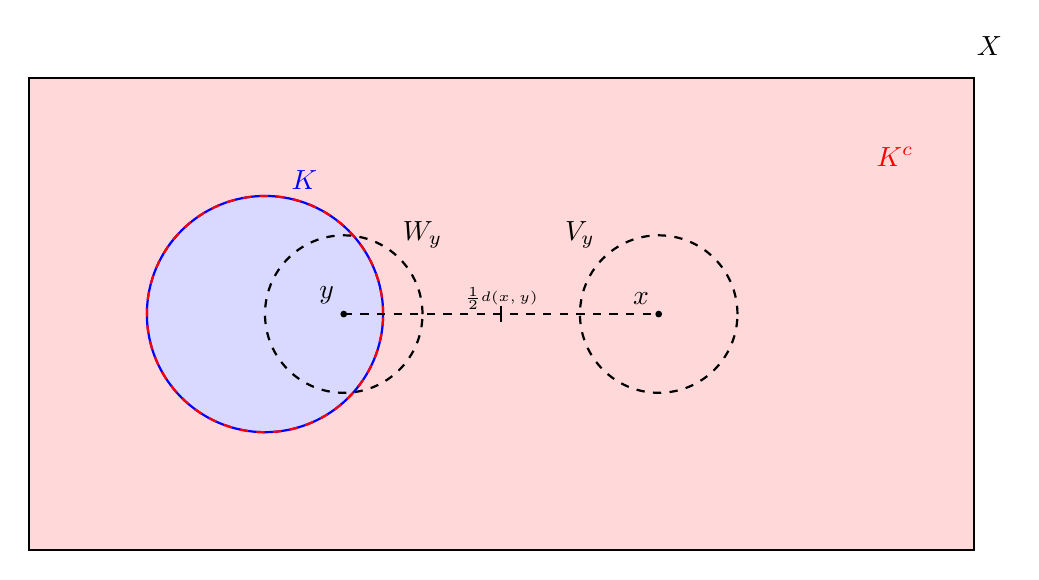
\begin{tikzpicture}
	\filldraw[color=black, thick, fill=red!15] (0,0) rectangle (12,6);
	\filldraw[color=blue, thick, fill=blue!15] (3,3) circle (1.5cm);
	\draw[thick, red, dashed, thick]  (3,3) circle (1.5cm);
	\draw[blue] (3.5,4.7) node {$ K $};
	\draw (12.2,6.4) node {$ X $};
	\draw[red] (11,5) node {$ K^c $};
	\filldraw (4,3) circle (1pt) node[anchor= south east] {$ y $};
	\filldraw (8,3) circle (1pt) node[anchor= south east] {$ x $};
	\draw[thick, dashed] (4,3) circle (1cm);
	\draw[thick, dashed] (8,3) circle (1cm);
	\draw[thick, dashed] (4,3) -- (8,3);
	\draw[thick] (6,3.1)--(6,2.9);  
	\draw[black] (6,3.2) node {\tiny$ \frac{1}{2}d(x,y) $};
	\draw[black] (5,4) node {$ W_{y}$};
	\draw[black] (7,4) node {$ V_{y}$};
	\end{tikzpicture}
	\caption{For some points $ x\in K^c $ and $ y\in K $, we construct neighborhoods $ W_y=N_r(y)$ and $ V_y=N_r(x) $ such that $ r<\frac{1}{2}d(x,y) $. This choice of radius ensures $ V_y\cap W_y=\emptyset $.}  
\end{figure}
 \begin{figure}[h!]
	\centering
	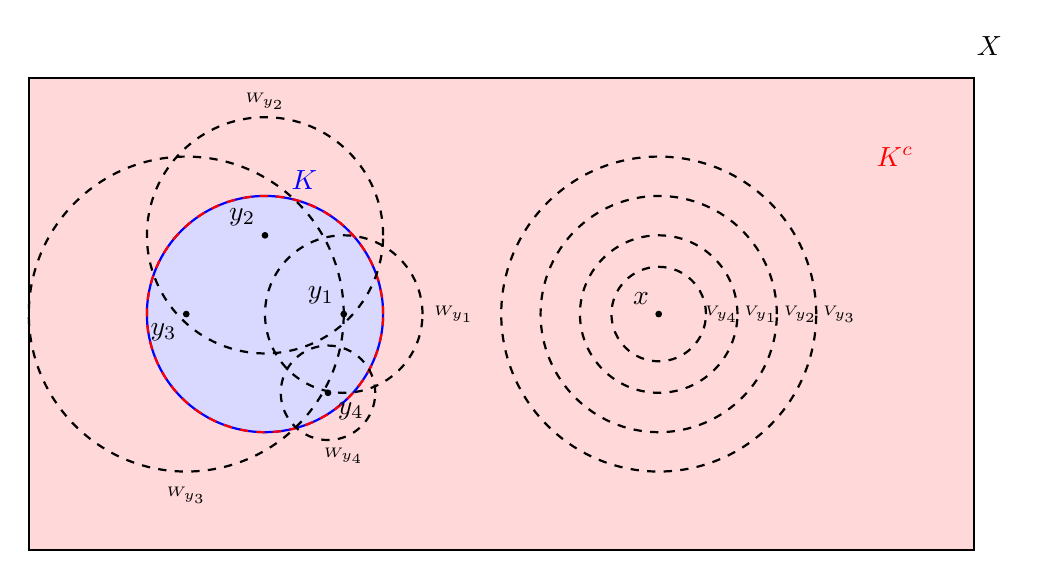
\begin{tikzpicture}
	\filldraw[color=black, thick, fill=red!15] (0,0) rectangle (12,6);
	\filldraw[color=blue, thick, fill=blue!15] (3,3) circle (1.5cm);
	\draw[thick, red, dashed, thick]  (3,3) circle (1.5cm);
	\draw[blue] (3.5,4.7) node {$ K $};
	\draw (12.2,6.4) node {$ X $};
	\draw[red] (11,5) node {$ K^c $};
	\filldraw (4,3) circle (1pt) node[anchor= south east] {$ y_1 $};
	\filldraw (8,3) circle (1pt) node[anchor= south east] {$ x $};
	\draw[thick, dashed] (4,3) circle (1cm);
	\draw[thick, dashed] (8,3) circle (1cm);
		\draw[thick, dashed] (8,3) circle (2cm);
				\draw[thick, dashed] (8,3) circle (0.6cm);
		\draw[thick, dashed] (3.8,2) circle (0.6cm);
	\draw[thick, dashed] (8,3) circle (1.5cm);
	\filldraw (3,4) circle (1pt) node[anchor= south east] {$ y_2 $}; 
		\filldraw (2,3) circle (1pt) node[anchor= north east] {$ y_3 $}; 
		\draw[thick, dashed] (2,3) circle (2cm);
		\draw[thick, dashed] (3,4) circle (1.5cm);
		\filldraw (3.8,2) circle (1pt) node[anchor= north west] {$ y_4 $};
		\draw[black] (8.8,3) node {\tiny$ V_{y_4}$};
		\draw[black] (9.3,3) node {\tiny$ V_{y_1}$};
		\draw[black] (9.8,3) node {\tiny$ V_{y_2}$};
		\draw[black] (10.3,3) node {\tiny$ V_{y_3}$};
		\draw[black] (4,1.2) node {\tiny$ W_{y_4}$};
		\draw[black] (5.4,3) node {\tiny$ W_{y_1}$};
		\draw[black] (3,5.7) node {\tiny$ W_{y_2}$};
		\draw[black] (2,0.7) node {\tiny$ W_{y_3}$};
		
	\end{tikzpicture}
	\caption{For the fixed value $ x\in K^c $, repeat the process illustrated in Figure 21 until we have a finite subcover of $ K $, $ \{W_{y_1},\ldots,W_{y_4}\}.$ If we let $ V $ be the intersection of all $ V_{y_i} $, then $ x\in V\subset K^c $, rendering $x $ an interior point of $ K^c $.}  
\end{figure}
\end{proof}
\begin{example}
	The set $ \Q $ in $ \R $ is not closed (Example 2.18), so it is not compact in $ \R $. 
\end{example}

\begin{theorem}
	Let $ X $ be a metric space, and $ K\subset X $ be compact. The set $ K $ is bounded. 
\end{theorem}
\begin{proof}
Let $ x\in K $. The collection of neighborhoods $ \{N_r(x)\} $ for $ r\in\N $ forms an open cover of $ K $. By compactness, this open cover has a finite subcover $ \{N_{r_1}(x),\ldots,N_{r_n}\} $. If we take $ r^*=\max\{r_1,\ldots,r_n\} $, then $ K\subset N_{r^*}(x) $, and $ d(x,y)<r^* $ for all $ y\in K $. (Figure 24)
  \begin{figure}[h!]
	\centering
	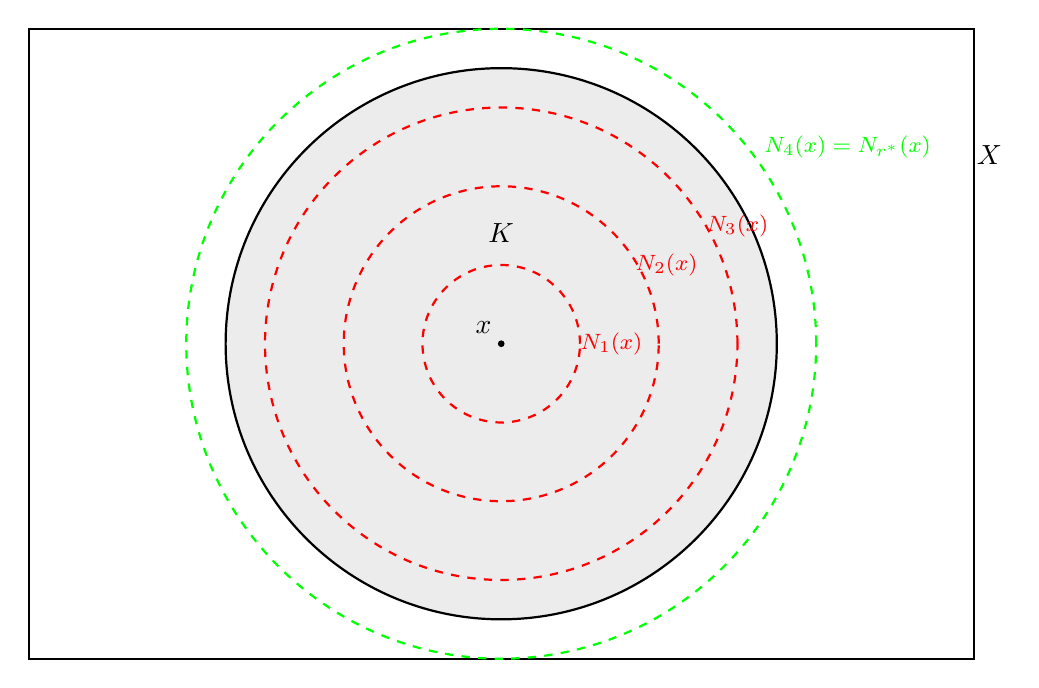
\begin{tikzpicture}
	\draw[color=black, thick] (0,0) rectangle (12,8);
	\filldraw[thick, fill=gray!15] (6,4) circle (3.5cm);
	\draw (12.2,6.4) node {$ X $};
	\draw (6,5.4) node {$ K $};
	\filldraw (6,4) circle (1pt) node[anchor = south east] {$ x $};
	\draw[thick, dashed, red] (6,4) circle (1cm);
	\draw[thick, dashed, red] (6,4) circle (2cm);
	\draw[thick, dashed, red] (6,4) circle (3cm);
	\draw[thick, dashed, green] (6,4) circle (4cm);	
	\draw[red] (7.4,4) node {\footnotesize$ N_{1}(x) $};
	\draw[red] (8.1,5) node {\footnotesize$ N_{2}(x) $};
	\draw[red] (9,5.5) node {\footnotesize$ N_{3}(x) $};
	\draw[green] (10.4,6.5) node {\footnotesize$ N_{4}(x)=N_{r^*}(x) $};
	\end{tikzpicture}
	\caption{We cover the set $ K $ with an infinite open cover comprised of neighborhoods of radii in $ \N $. By compactness there is an open subcover, such as $ \{N_1(x),\ldots,N_4(x)\} $. The set is bounded by the maximum radii $ r^*=4 $ in this finite collection.}  
\end{figure}
\end{proof}
\begin{example}
The set $ (0,\infty) $ in $ \R $ is not bounded so it is not compact in $ \R $. 
\end{example}
\begin{remark}
	While compactness implies closed and bounded, the converse \textit{is not necessarily true}. Soon, we will see that the converse will hold in $ \R^n $, but in general, this is not the case. The next example illustrates this.
\end{remark}
\begin{example}
	Let $ X=\{1/n\mid n\in\N\} $ be a metric space equipped with $$ d(x,y)=\begin{cases}
	0\text{ if }x=y\\1\text{ if }x\neq y
	\end{cases}.$$
The set $ X $ is closed, as it is the whole space. It is also bounded, as $ d(x,y)\le 1 $ for all $ x,y\in X $. Let $ G_n=\{1/n\} $. Each $ G_n $ is open, as $ N_{1/2}(1/n)\subset G_n $. This makes $ G_n $ an open cover of $ X $, as $ X\subset\bigcup_{n\in \N} G_n=X $. The set $ X $ fails to be compact, because this open cover has no finite subcover. Any finite cover $ \{G_{1},\ldots,G_{N}\} $ would not ``cover''  $ \{1/(N+1),1/(N+2),\ldots\}\subset X $.	
\end{example}

We often restrict our attention to subsets of compact sets, so it would be nice to know if subsets of compact sets are compact. Unfortunately, this is not true in general, but it becomes true if we require the subset satisfy one condition. 
\begin{proposition}
	Closed subsets of compact sets are compact.
\end{proposition}
\begin{proof}
	Suppose $ K $ in $ X $ is compact, and $ F\subset K $ is closed in $ X $. Let $ \{V_\alpha\} $ be an arbitrary open cover of $ F $. If we add $ F^c $ to this collection of open sets, we have an open cover $ \Omega=\{V_{\alpha_1},V_{\alpha_2},\ldots,F^c\} $ of $ K $, because $ K=F\cup F^c $. $$ K\subset\left(\bigcup_\alpha V_\alpha\right)\cup F^c.$$ The set $ K $ is compact, so there exists a finite open cover of $ \Omega $, $ \Phi=\{V_{\alpha_1},\ldots,V_{\alpha_n}, F^c\} $. We can now remove $ F^c $ from $ \Phi $, resulting in a finite subcover for $ \{V_\alpha\} $. 
\end{proof}
\begin{corollary}
	If $ F $ is closed and $ K $ is compact, $ F\cap K $ is compact. 
\end{corollary}
An interesting property of compact sets is that if we have a decrease sequence of nested compact intervals, than their intersection is nonempty. This result follows as a corollary of a more general result.
\begin{proposition}
	If $ \{K_\alpha\} $ is a collection of compact subsets of a metric space $ X $ such that the intersection of every finite subcollection of $ \{K_\alpha\} $ is nonempty, then $ \cap_\alpha K_\alpha\neq\emptyset $. 
\end{proposition}
\begin{proof}
For the sake of contradiction, assume that $ \cap_\alpha K_\alpha=\emptyset $. This means there is some fixed $K_1\in \{K_\alpha\}$ such that no point of $ K_1 $ belongs to every $ K_\alpha $. Let $ G_\alpha= K_\alpha^c $. The collection $ \{G_\alpha\} $ forms an open cover of $ K_1$. Since $ K_1 $ is compact, there exists a finite subcover $ \{G_{\alpha_1},\ldots,G_{\alpha_n}\} $. $$ K\subset\bigcup_{i=1}^nG_{\alpha_i}$$ This inclusion, along with the definition of $ G_\alpha $ implies that $ K_1\cap\left(\bigcap_{i=1}^nK_{\alpha_i}\right)=\emptyset $. This contradicts our assumption that every finite subcollection of $ \{K_\alpha\} $ is nonempty. 
\end{proof}
\begin{corollary}[Cantor's Intersection Theorem]
If $ \{K_\alpha\} $ is a sequence of nonempty compact sets such $ K_{n}\supset K_{n+1} $ for $ n\in\N $, then $ \cap_{i=1}^\infty K_n $ is not empty.
\end{corollary}
\begin{example}
	Recall that open intervals in $ \R $ are not compact (Example 2.35), and do not satisfy the requirement of Cantor's Intersection Theorem. Let $ G_{n}=(0,1/n) $. We have $ G_{n+1}\subset G_{n} $ for all $ n\in\N $, so $ \{G_n\} $ is a decreasing nested sequence of intervals. $$ \cdots\subset \left(0,\frac{1}{4}\right)\subset\left(0,\frac{1}{3}\right)\subset\left(0,\frac{1}{4}\right)\subset\left(0,\frac{1}{2}\right)\subset(0,1)$$  
The intersection of these sets is empty.	
\end{example}
\begin{proposition}[Bolzano-Weierstrass Property]
	If $ E $ is an infinite subset of a compact set $ K $, then $ E $ has a limit point in $ K $. 
\end{proposition}
\begin{proof}
	For the sake of contradiction, assume that no point of $ K $ is a limit point of $ E $. For each $ x\in K $, there exists some $ r $ such that $ V_x=N_r(x)=\{x\}  $ if $ x\in E $, or $ V_x=N_r(x)=\emptyset $ if $ x\notin E $. The collection $ \{V_x\} $ is an open cover of $ E $. The set $ E $ is infinite, so we cannot find a finite subcover for $ \{V_x\} $, as each set is at most a singleton. Because $ E\subset K $, the same is true with respect to $ K $, which contradicts the assumption that $ K $ is compact. 
\end{proof}
Informally, the Bolzano-Weierstrass Property tells us that we can approximate some point of $ K $ with points in an infinite subset $ E $. Right now, this may not seem significant, but it will become important when we work in $ \R^n $. 
\begin{remark}
	The Bolzano-Weierstrass Property is often referred to as \textit{\color{red}limit point compactness}. In the context of metric spaces, limit point compactness and compactness are equivalent\footnote{Proving this requires some concepts that are beyond this treatment of metric spaces.}, so in most real analysis texts the prior is never even given a name. As we'll see \textit{much} later on, the two are not equivalent when we explore point-set topology in general (Section 19).   
\end{remark} 
\subsection{Compact Sets in $ \R^n $}
Now we can start working towards sufficient conditions for compactness in $ \R^n $. This will culminate in the famed Heine-Borel Theorem. This theorem establishes sufficient conditions for compactness in $ \R^n $. Specifically, the converses of Theorem 2.3 and Theorem 2.4 will hold in $ \R^n $.  

In order to make the proof of this result a bit more clear, we will show a series of results beforehand which build to the Heine-Borel Theorem.
\begin{lemma}
	If $ \{I_n\} $ is a sequence of closed intervals in $ \R $, such that $ I_n\supset I_{n+1} $  for $ n\in\N $, then $ \cap_{i=1}^n I_n\neq\emptyset$.
\end{lemma}  
		\begin{figure}[h]
	\centering
	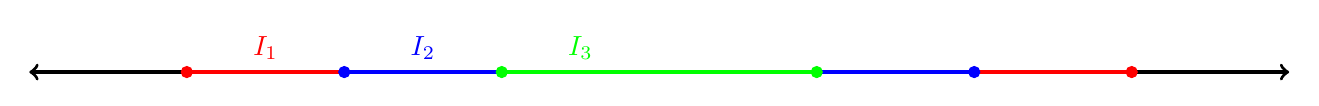
\begin{tikzpicture}
	\draw[very thick, <->] (-8,0) -- (8,0);
	\filldraw[fill=red, color=red] (-6,0)circle (2pt);
	\filldraw[fill=red, color=red] (6,0) circle (2pt);
	\draw[very thick, color = red] (-6,0)--(6,0);
	\draw[red] (-5,.3) node {$ I_1$};
		\filldraw[fill=blue, color=blue] (-4,0)circle (2pt);
	\filldraw[fill=blue, color=blue] (4,0) circle (2pt);
	\draw[very thick, color = blue] (-4,0)--(4,0);
	\draw[blue] (-3,.3) node {$ I_2$};
		\filldraw[fill=green, color=green] (-2,0)circle (2pt);
	\filldraw[fill=green, color=green] (2,0) circle (2pt);
	\draw[very thick, color = green] (-2,0)--(2,0);
	\draw[green] (-1,.3) node {$ I_3$};
	\end{tikzpicture}
	\caption{The first three intervals in the type of sequence $ \{I_n\} $ described in Proposition 2.7.}
\end{figure}
\begin{proof}
	Suppose $ I_n=[a_n,b_n] $. Define $ E $ to be the set of all the $ a_n $. The set $ E $ is nonempty and bounded above by $ b_1 $, because $$\cdots a_3\le a_2\le a_1\le b_1\le b_2\le b_3\le \cdots .$$ We have $ E\subset \R $ and is bounded, so it has a supremum in $ \R $. Let $ x=\sup E $. For all $ m,n\in\N $, $$a_n\le a_{m+n}\le b_{m+n}\le b_m ,$$ so $ x\le b_m $ for all $ m $. By the definition of $ \sup E $, $ a_m\le x $. If $ x\le b_m $ and $ a_m\le x $, then $ x\in[a_m,b_m]=I_m $ for all $ m\in\N $. Therefore $ x\in\cap_{n\in\N} I_n $.
\end{proof}
\begin{example}
	If we modify Example 2.42 so the open intervals are closed, then we have a sequence $ \{I_n\} $ where $ I_n=[0,1/n] $. This gives $ \cap_{n\in\N} I_n=\{0\}\neq\emptyset $. If we worked through the proof of Lemma 2.2 with this particular example, we would find that $ 0 $ is the supremum of the set of lower bounds of $ I_n $. 
\end{example}
This result should look familiar. Cantor's Intersection Theorem states a similar result for compact sets. This in and of itself does not show that closed intervals are compact, but it should catch our attention, as closed intervals and compact sets share a noteworthy property. It should also be noted that this property of closed intervals follows from the least-upper-bound property of $ \R $. This is one of the magical results we get because $ \R $ is complete.  We can generalize Proposition 2.7 to \textit{\color{red}$ k $-cells} in $ \R^k $. An  $ k $-cell is the set of all points $ \x=(x_1,\ldots,x_k)\in\R^k $ which satisfy $ a_i\le x_i\le b_i $ for $ i=1,\ldots,k $, where $ a_i,b_i\in\R $, and $ a_i\le b_i $. 
\begin{lemma}
	Let $ k\in\N $. If $ \{I_n\} $ is a sequence of $ k- $cells such that $ I_n\supset I_{n+1} $ for all $ n\in\N $, then $ \cap_{n\in\N} I_n\neq\emptyset $. 
\end{lemma}
		\begin{figure}[h]
	\centering
	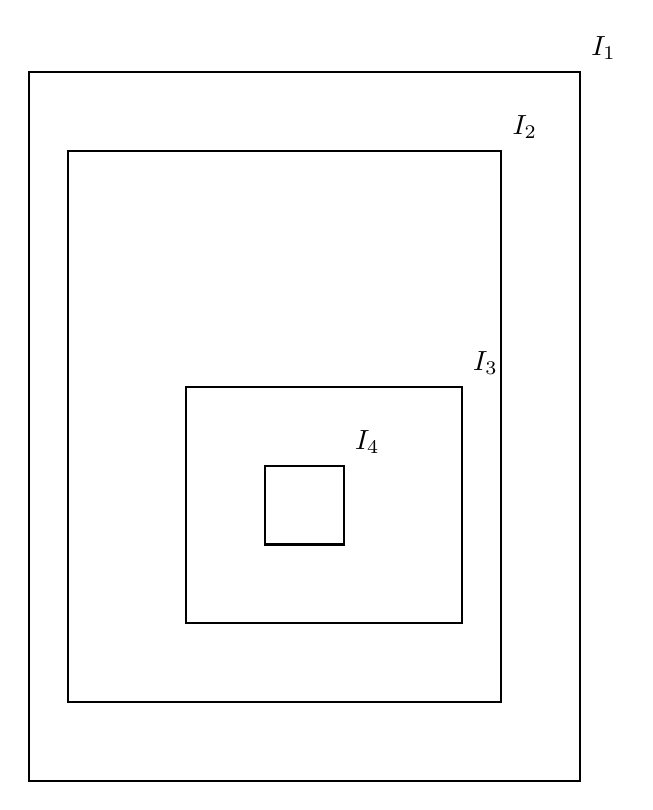
\begin{tikzpicture}
\draw[thick] (0,0) rectangle (7,9);
\draw (7.3,9.3) node {$ I_1$};
\draw[thick] (0.5,1) rectangle (6,8);
\draw (6.3,8.3) node {$ I_2$};
\draw[thick] (2,2) rectangle (5.5,5);
\draw (5.8,5.3) node {$ I_3$};
\draw[thick] (3,3) rectangle (4,4);
\draw (4.3,4.3) node {$ I_4$};
	\end{tikzpicture}
	\caption{The first four $ 2- $cells in the type of sequence $ \{I_n\} $ described in Proposition 2.8.}
\end{figure}
\begin{proof}
	Let $ I_n $ be the set of points $ \x=(x_1,\ldots,x_k) $ such that $ a_{n,j}\le x_j\le b_{n,j} $ for $ j=1,\ldots, k $ and $ n\in\N $, and write $ I_{n,j}=[a_{n,j},a_{b,j}] $. By Lemma 2.2, for each $ I_{n,j} $, $ \cap_{n\in\N}I_{n,j}\neq\emptyset $, so there is some $ x_j^*\in\cap_{n\in\N} I_{n,j} $ which satisfies $$ a_{n,j}\le x_j^*\le b_{n,j}$$ for $j=1,\ldots, k $ and $ n\in\N $. If we set $ \x^*=(x_1^*,\ldots,x_k^*) $, then $ \x^*\in I_n $ for all $ n\in\N $. Therefore  $ \cap_{n\in\N} I_n\neq\emptyset $. 
\end{proof}
We will now prove that each $ k -$cell is compact. The definition of a $ k -$cell is equivalent to a closed and bounded set in $ \R $, so this result will give us our sufficient conditions for compactness in $ \R^n $. This result will give rise to the Heine-Borel Theorem which is an equivalence result, which will follow immediately from the compactness of $ k $-cells, Theorem 2.3, and Theorem 2.4. That being said, the proof that each $ k -$cell is compact is not immediate, and is on the more difficult side for a proof in an introductory analysis course.    
\begin{lemma}
	Every $ k -$cell is compact. 
\end{lemma}
\begin{proof}
	Let $ I=\{\x\in\R^k\mid a_j\le x_j\le b_j\ j=1,\ldots,k\} $ be a $ k- $cell. Let $ \delta $ be the maximum distance between any two points in $ I $.
	$$ \max\limits_{\x,\y\in I}d(\x,\y)=\delta=\left(\sum_{j=1}^k(b_j-a_j)^2\right)^{1/2}$$
	For all $ \x,\y\in I $, $ |\x-\y|\le\delta $ (Figure 27 shows this for $ k=2 $). 
			\begin{figure}[h!]
		\centering
		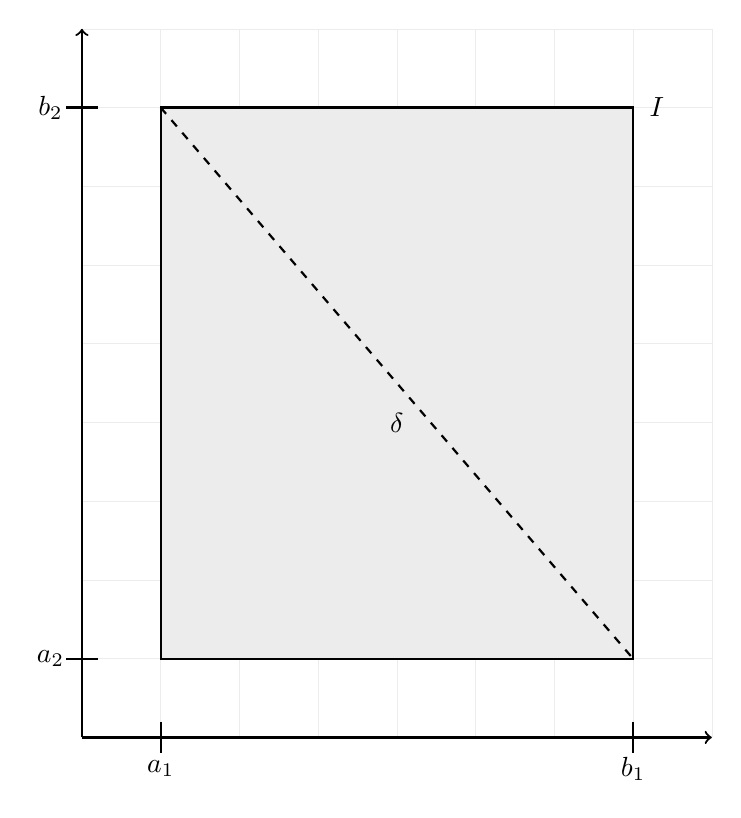
\begin{tikzpicture}
	
		\draw[step=1cm,gray!15,very thin] (0,0) grid (8,9);
		\filldraw[thick, fill = gray!15] (1,1) rectangle (7,8);
		\draw (7.3,8) node {$ I$};	
		\draw[thick,->] (0,0) -- (0,9);
		\draw[thick,->] (0,0) -- (8,0);
		\draw[thick] (1,0.2) -- (1,-0.2);
		\draw[thick] (7,0.2) -- (7,-0.2);
		\draw[thick] (-0.2,1) -- (0.2,1);
		\draw[thick] (-0.2,8) -- (0.2,8);
		\draw (1,-0.4) node {$ a_1$};	
		\draw (7,-0.4) node {$ b_1$};
		\draw (-0.4,1) node {$ a_2$};
		\draw (-0.4,8) node {$ b_2$};
		\draw[thick, dashed] (1,8) -- (7,1) ;
		\draw (4,4) node {$ \delta $};
		\end{tikzpicture}
		\caption{If $ I $ is a 2-cell.}
	\end{figure}

For the sake of contradiction, assume that there exists some arbitrary open cover $ \{G_\alpha\} $ of $ I $ which contains no finite subcover of $ I $. Let $ c_j=(a_j+b_j)/2 $. The intervals $ [a_j,c_j] $ and $ [c_j,b_j] $ give rise to $ 2^k $ $ k $-cells $ Q_i $ whose union is $ I $. If each of these cells $ Q_i $ could be covered by a finite subcollection of $ \{G_\alpha\} $, then $ I $ could be covered by the union of all these finite subcollections, which is finite. Since we've assumed $ K $ is not compact, then it must be that there exists at least one $ Q_i $, call it $ I_1 $, that cannot be covered by any finite subcollection of $ \{G_\alpha\} $.  
	\begin{figure}[h!]
	\centering
	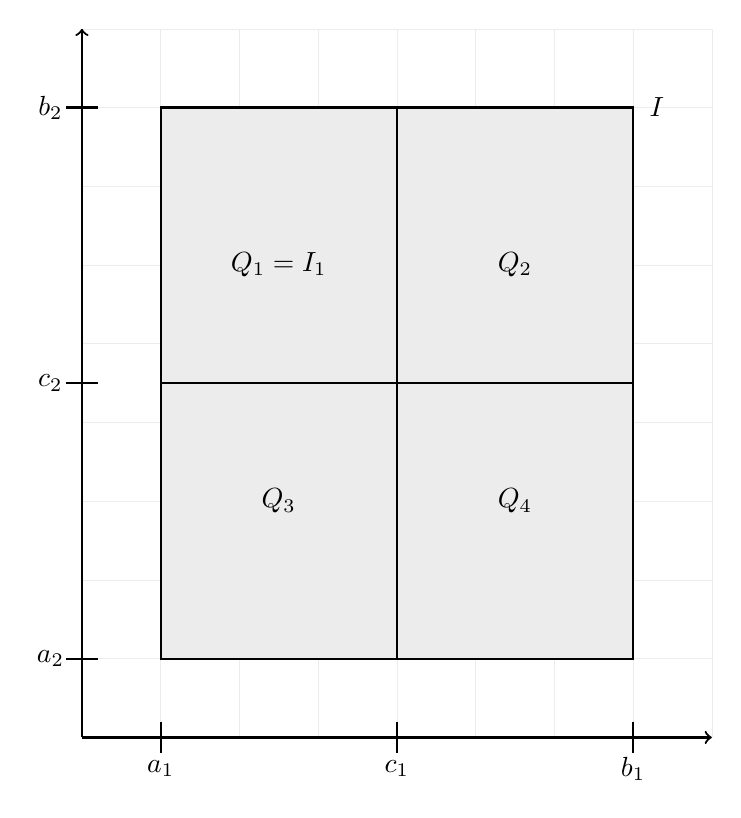
\begin{tikzpicture}
	
	\draw[step=1cm,gray!15,very thin] (0,0) grid (8,9);
	\filldraw[thick, fill = gray!15] (1,1) rectangle (7,8);
	\draw (7.3,8) node {$ I$};	
	\draw[thick,->] (0,0) -- (0,9);
	\draw[thick,->] (0,0) -- (8,0);
	\draw[thick] (1,0.2) -- (1,-0.2);
	\draw[thick] (7,0.2) -- (7,-0.2);
	\draw[thick] (-0.2,1) -- (0.2,1);
	\draw[thick] (-0.2,8) -- (0.2,8);
	\draw (1,-0.4) node {$ a_1$};
	\draw (4,-0.4) node {$ c_1$};	
	\draw (7,-0.4) node {$ b_1$};
	\draw (-0.4,1) node {$ a_2$};
	\draw (-0.4,8) node {$ b_2$};
	\draw (-0.4,4.5) node {$ c_2$};
	\draw[thick] (-0.2,4.5) -- (0.2,4.5);
	\draw[thick] (4,0.2) -- (4,-0.2);
	\draw[thick] (1,4.5)-- (7,4.5);
	\draw[thick] (4,1)-- (4,8);
	\draw (2.5,3) node {$ Q_3$};
	\draw (5.5,3) node {$ Q_4$};
	\draw (2.5,6) node {$ Q_1=I_1$};
	\draw (5.5,6) node {$ Q_2$};
	\end{tikzpicture}
	\caption{We partition $ I $ into $ 2^k $ cells $ Q_i $. If $ I $ is not compact, then there is some $ Q_i $ which is not compact. Suppose in this case $ Q_1 $ is not compact, and call it $ I_1 $. }
\end{figure}
Now we divide $ I_1 $ into $ 2^k $ $ k -$cells and repeat this process indefinitely, giving us a sequence $ \{I_n\} $ (Figure 29). 
	\begin{figure}[h!]
	\centering
	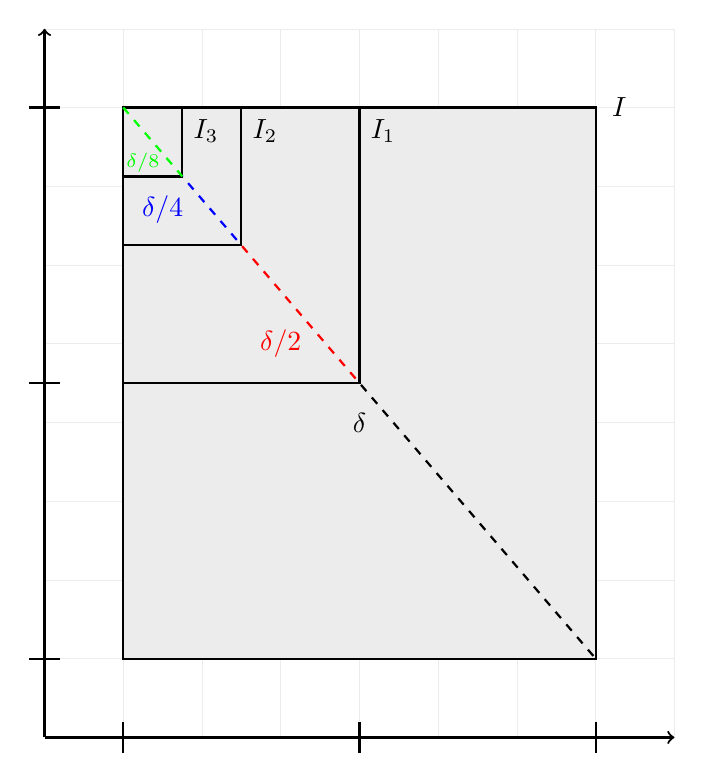
\begin{tikzpicture}
	
	\draw[step=1cm,gray!15,very thin] (0,0) grid (8,9);
	\filldraw[thick, fill = gray!15] (1,1) rectangle (7,8);
	\draw (7.3,8) node {$ I$};	
	\draw[thick,->] (0,0) -- (0,9);
	\draw[thick,->] (0,0) -- (8,0);
	\draw[thick] (1,0.2) -- (1,-0.2);
	\draw[thick] (7,0.2) -- (7,-0.2);
	\draw[thick] (-0.2,1) -- (0.2,1);
	\draw[thick] (-0.2,8) -- (0.2,8);

	\draw[thick, dashed] (1,8) -- (7,1) ;

	\draw (4,4) node {$ \delta $};
	\draw[thick] (-0.2,4.5) -- (0.2,4.5);
	\draw[thick] (4,0.2) -- (4,-0.2);
	\filldraw[thick, fill = gray!15] (1,4.5) rectangle (4,8);	
	\draw[thick, dashed, red] (1,8) -- (4,4.5) ;
	\filldraw[thick, fill = gray!15] (1,6.25) rectangle (2.5,8);
	\draw[thick, dashed, blue] (1,8) -- (2.5,6.25) ;
	\filldraw[thick, fill = gray!15](1,7.125) rectangle (1.75,8);
	\draw[thick, dashed, green] (1,8) -- (1.75,7.125) ;
	\draw (4.3,7.7) node {$ I_1$};
	\draw (2.8,7.7) node {$ I_2$};
	\draw (2.05,7.7) node {$ I_3$};
	\draw[red] (3,5) node {$ \delta/2 $};
\draw[blue] (1.5,6.7) node {$ \delta/4 $};
\draw[green] (1.25,7.3) node {\scriptsize$ \delta/8 $};
	\end{tikzpicture}
	\caption{The first three $ 2 $-cells in the sequence $ \{I_n\} $.}
\end{figure}
This sequence of $ k $-cells was constructed to have three properties:
\begin{enumerate}
	\item $ I\supset I_1\supset I_2\supset I_3\supset\cdots $
	\item $ I_n $ cannot be covered by any finite subcollection of $ \{G_\alpha\} $, otherwise $ K $ would not be compact.\footnote{This follows from the same reasoning applied to the $ 2^k $ $ k $-cells $ Q_i $ we initially chose $ I_1 $ from.}
	\item If $ \x,\y\in I_n $, then $ |\x-\y|\le \delta/2^n $.\footnote{When we divided $ I $, the length of the diagonal for $ I_1 $ became half of $ \delta $. When we divide $ I_1 $, the length of the diagonal of $ I_2 $ became half of that of $ I_1 $. This means we can always write the diagonal of $ I_n $ in terms of powers of $ 1/2 $ and $ \delta $.  }
\end{enumerate}
By the first property of this sequence, we can invoke Lemma 2.3 to determine $ \cap_{n\in\N} I_n\neq\emptyset $. This means there exists some $ \x^*\in\R^k $ such that $ \x^*\in I_n $ \textit{for all} $ n\in\N $. There must be some $ \alpha $ such that $ \x^*\in G_\alpha $, otherwise $ \{G_\alpha\} $ would not be an open cover of $ I $. Since $ G_\alpha $ is open, there exists some $ r>0 $ such that $ N_r(x)\subset G_\alpha $. Alternatively, we could say that $ |\y-\x^*|<r $ implies $ y\in G_\alpha $ by the definition of $ N_r(x) $. If we take $ n $ to be so large that $ \delta/2^n<r $, then $ I_n\subset G_\alpha $, but this would mean $ I_n $ has a finite subcover. This contradicts property $ 2 $ of our sequence $ \{I_n\} $, thereby contradicting the assumption that $ K $ is not compact. 
\end{proof}
We have now shown that every $ k $-cell is compact. The proof is made more manageable with illustrations, but is still rather technical. Our contradiction came from the fact that as $ n $ becomes large, $ I_n $ becomes small. Eventually $ I_n $ will be so small, that it must have a finite open subcover. This contradicts the assumption that $ I $ is not compact. 
\begin{theorem}[Heine-Borel Theorem]
	A set $ E $ in $ \R^n $ is compact \textit{if and only if} it is closed and bounded.
\end{theorem} 
\begin{proof}{\color{white}space}
\begin{enumerate}
	\item [$ (\Longrightarrow) $] All compact sets are closed and bounded by Theorems 2.3 and 2.4. 
	\item [$ (\Longleftarrow) $] If $ E $ is closed and bounded then $ E\subset I $ for some $ n -$cell. Any closed subset of a compact set is compact by Proposition 2.4, so $ E $ is compact.
\end{enumerate}
\end{proof}
\begin{example}
	Any closed interval $ [a,b]\subset \R$ is compact. 
\end{example}
\begin{theorem}[Bolzano–Weierstrass Theorem]
	Every bounded infinite subset of $ \R^n $ has a limit point in $ R^k $. 
\end{theorem}
\begin{proof}
	Let $ E\subset\R^n $ be bounded and infinite. There is some $ n $-cell $ I\subset\R^k $, such that $ E\subset I $. By Lemma 2.4 $ I $ is compact. We know apply Proposition 2.6 to conclude that $ E $ has a limit point in $ I $, which is also in $ \R^k $.
\end{proof}
\begin{example}
	The set $ (a,b)\subset\R^n $ is infinite and bounded. It has an infinite number of limit points in $ \R^n $,\footnote{In fact, the set of limit points is $ [a,b]\subset\R^n $} including $ a $ and $ b $.
\end{example}
\subsection{Exercises}
\begin{ex}
	Show that the set of all algebraic numbers is countably infinite.
\end{ex}
\begin{ex}
	Show that the set of all binary numbers with infinite digits is uncountably infinite.
\end{ex}
\begin{ex}
	Verify that the taxi-cab metric on $ \R^n $ is a valid metric space.
\end{ex}
\begin{ex}
	Let $ X $ be an infinite set with the metric, $$d(x,y)=\begin{cases}
		1\text{ if }x\neq y\\
	0\text{ if }x=y
	\end{cases} .$$ Prove that $ (X,d) $ is a metric space. Which subsets of $ X $ are open? Which are closed? 
\end{ex}
\begin{ex}
	Prove that $ E^\circ $ is open.
\end{ex}
\begin{ex}
	Prove that $ E $ is open \textit{if and only if} $ E=E^\circ $.
\end{ex}
\begin{ex}
	If $ G\subset E $ and $ G $ is open, prove that $ G\subset E^\circ $
\end{ex}
\begin{ex}
	Prove that $ (E^\circ)^c=\overline{E^c} $.
\end{ex}
\begin{ex}
	Find an example of a set $ E  $ in a metric space such that $ E^\circ\neq(\bar{E} )^\circ$.
\end{ex}
\begin{ex}
	Find an example of a set $ E  $ in a metric space such that $ \bar{E}\neq\overline{E^\circ}$.
\end{ex}
\begin{ex}
	Prove that $ \partial E $ is closed.
\end{ex}
\begin{ex}
	Prove that $ \partial(E^\circ)\subset \partial E  $, and $ \partial(\bar{E})\subset \partial E  $
\end{ex}
\begin{ex}
	Prove that $ \partial E=\partial (E^c)  $.
\end{ex}
\begin{ex}
	Suppose $ E $ is closed. Show that $ (\partial E)^\circ=\emptyset $. 
\end{ex}
\begin{ex}
	Prove that $ \partial (\partial E)\subset \partial E $. When will the sets be equal? 
\end{ex}
\begin{ex}
	Prove that $ E $ is closed \textit{if and only if} $ E\cap \partial E=\emptyset $.
\end{ex}
\begin{ex}
	Prove that $ \partial E=\emptyset$ \textit{if and only if} $ E $ is closed and open.  
\end{ex}
\begin{ex}
	Prove that $ \bar{E}=E\cup\partial E $.
\end{ex}
\begin{ex}
	Prove that $ (\partial \bar{E})^\circ=\emptyset $. 
\end{ex}
\section{Sequences and Series}
\subsection{Convergence}
density
\subsection{Subsequences}
\subsection{Cauchy Sequences}
\subsection{Extending $ \R $}
\subsection{$ \limsup $ and $ \liminf $}
\subsection{Series}

\section{Continuity}
\subsection{Limits of Functions}
\subsection{Continuous Functions}
\subsection{Intermediate Value Theorem}
\subsection{Uniform Continuity}
\subsection{Continuity and Compactness}
\subsection{Discontinuities}
\subsection{Monotonicity}
\section{Differentiation}
\subsection{The Definition of a Derivative}
\subsection{Properties of the Derivative}
\subsection{The Chain Rule}
\subsection{Mean Value Theorem}
\subsection{L'H\^{o}pital's Rule}
\section{Riemann Integration}
\subsection{Partitions}
\subsection{Simple Functions}
\subsection{Upper and lower Riemann Integrals}
\subsection{Properties of the Riemann Integral}
\subsection{Integration with Continuity and/or Monotonicity}
\subsection{Riemann-Stieltjes Integral}
\section{Sequences and Series of Functions}
\subsection{Spaces of Functions}
\subsection{Sequences}
\subsection{Convergence}
\subsection{Uniform Convergence}
\subsection{Properties of Uniform Convergence}
\subsection{Series}
\subsection{Power Series}
\subsection{Taylor Series}
\section{Functions of Several Variables}
\subsection{Linear Transformations}
\section{Differentiation with Several Variables}
\subsection{The Derivative as a Linear Map}
\subsection{The Chain Rule}
\subsection{The Inverse Function Theorem}
\subsection{The Implicit Function Theorem}
\section{Riemann Integration with Several Variables}
\subsection{Integration over a Rectangle}
\subsection{Iterated Integrals}
\subsection{Change of Variables}
\subsection{Change of Variables, Proof}
\section{Differential Forms}
\subsection{Motivation and Review of Vector Calculus}
\subsection{Tensors}
\subsection{Wedge Product}
\subsection{Tangent Vectors and Differential Forms}
\subsection{Manifolds}
\subsection{Stokes' Theorem}
\section{Measures}
\subsection{Motivation}
\subsection{$ \sigma $-Algebras}
\subsection{Measures}
\subsection{Outer Measures}
\subsection{Measures on $ \R $}
\section{Integration Revisited}
\subsection{Measurable Functions}
\subsection{Itegration of Simple Functions}
\subsection{Integration of Nonnegative Functions}
\subsection{Integration of Real Functions}
\subsection{Product Measures}
\subsection{Lebesgue Integration in $ n- $Dimensions}
\section{Differentiation with Measures}
\subsection{Motivation in $ \R $}
\subsection{Signed Measures}
\subsection{Radon-Nikodym Derivative}
\section{Foundations of Functional Analysis}
\subsection{Normed Vector Spaces}
\subsection{Linear Functionals}
\subsection{The Baire Category Theorem}
\subsection{Hilbert Spaces}
\section{$ L^p $ Spaces}
\subsection{Basic Theory}
\subsection{The Dual of $ L^p $}
\subsection{Inequalities}
\section{Radon Measures}
\section{Foundations of Fourier Analysis}
\section{Point-Set Topology}
\subsection{Topological Spaces}
\subsection{Nets}
\subsection{Filters}
\subsection{Various Notions of Compactness}
\subsection{Continuity}
\subsection{The Product Topology}
\subsection{Pointwise and Uniform Convergence}
\newpage
\bibliography{analysis}{} 
\end{document}